
\section{Two $b$-Tag Samples}

	



\begin{figure} % "[t!]" placement specifier just for this example
	\centering	
	\begin{subfigure}{0.25\textwidth}
		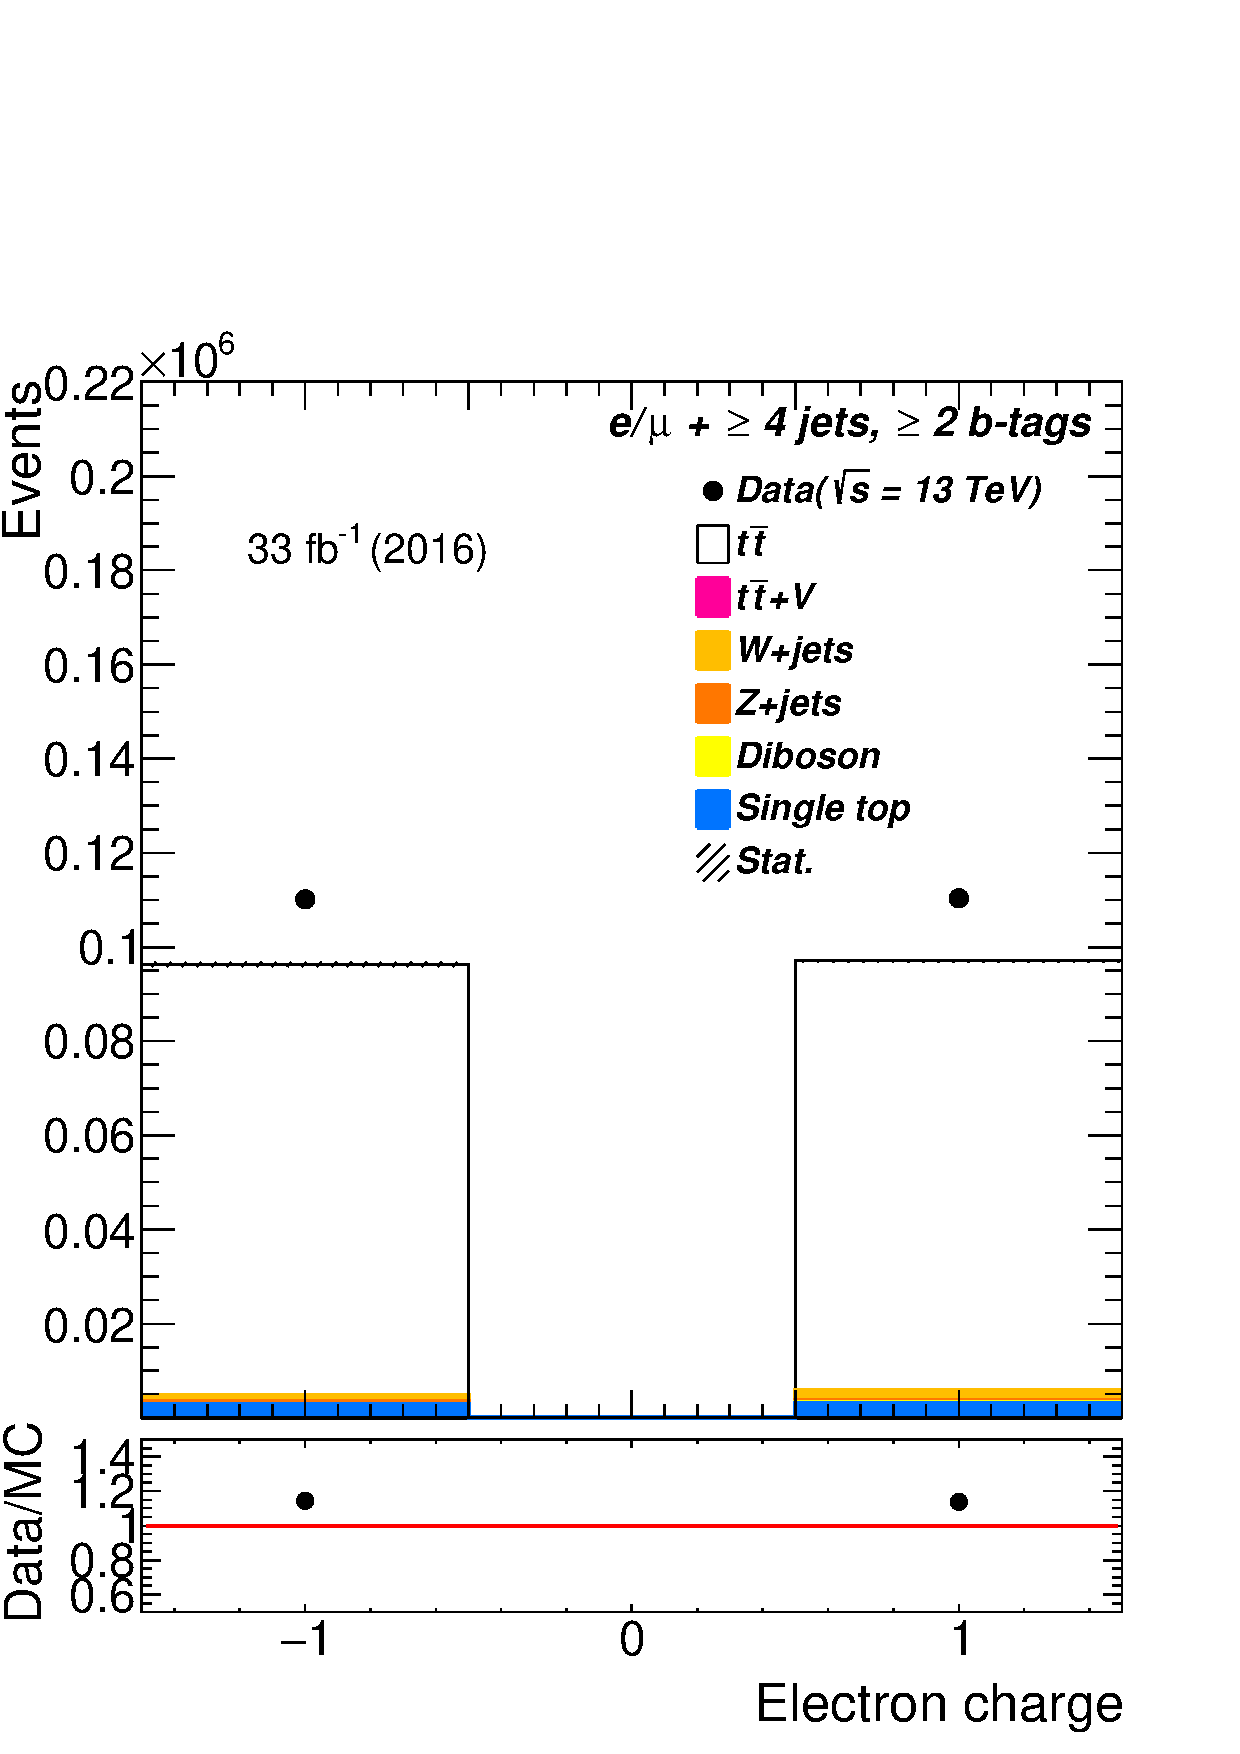
\includegraphics[width=\linewidth]{ControlPlots_emujets_2016_4incl_2incl/el_charge_emujets_2016.png}
		\caption{Electron charge.} \label{fig:a1}
	\end{subfigure}\hspace*{1.0cm}
	\begin{subfigure}{0.25\textwidth}
		\includegraphics[width=\linewidth]{ControlPlots_emujets_2016_4incl_2incl/el_n_emujets_2016.png}
		\caption{Number of electrons.} \label{fig:b1}
	\end{subfigure}\hspace*{1.0cm}
	\begin{subfigure}{0.25\textwidth}
		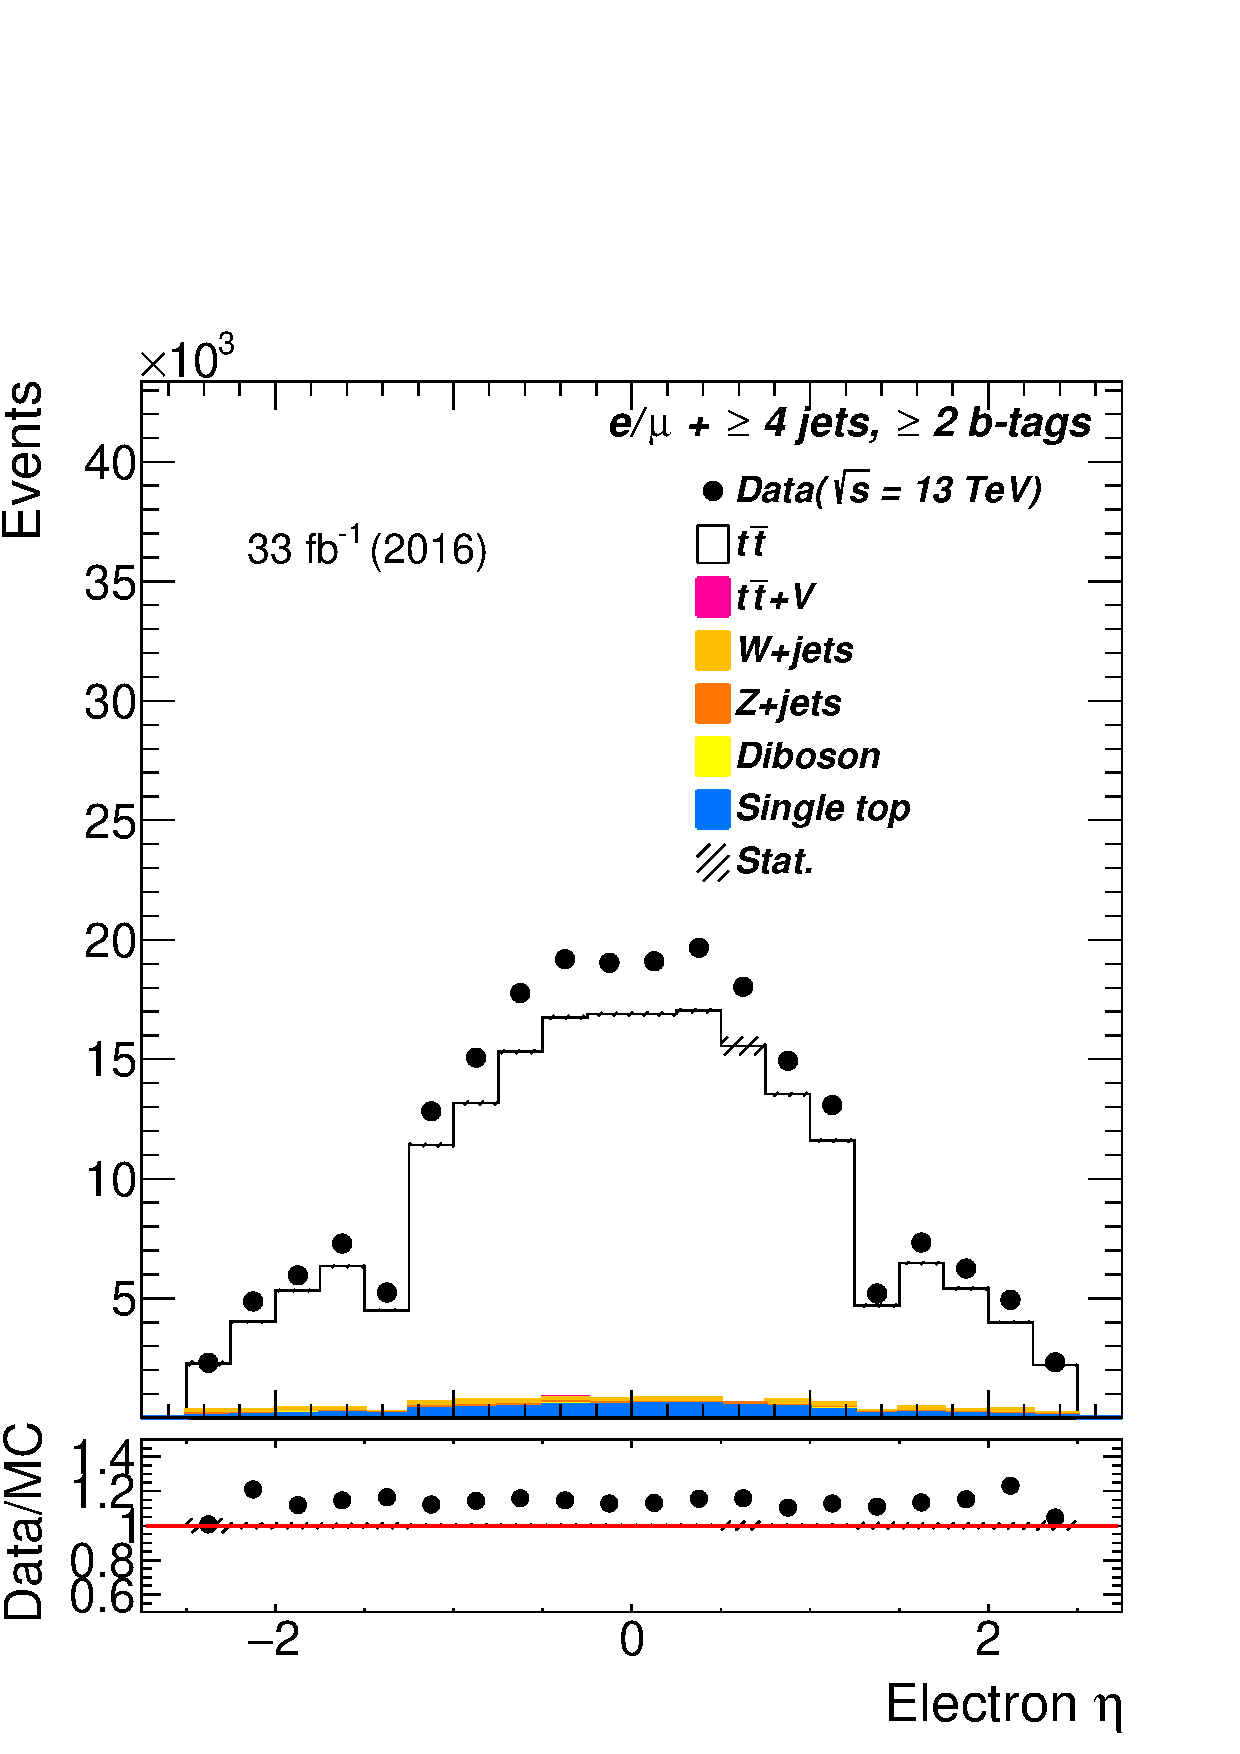
\includegraphics[width=\linewidth]{ControlPlots_emujets_2016_4incl_2incl/el_eta_emujets_2016.png}
		\caption{Rapidity of the electrons.} \label{fig:c1}
	\end{subfigure}
	\begin{subfigure}{0.25\textwidth}
		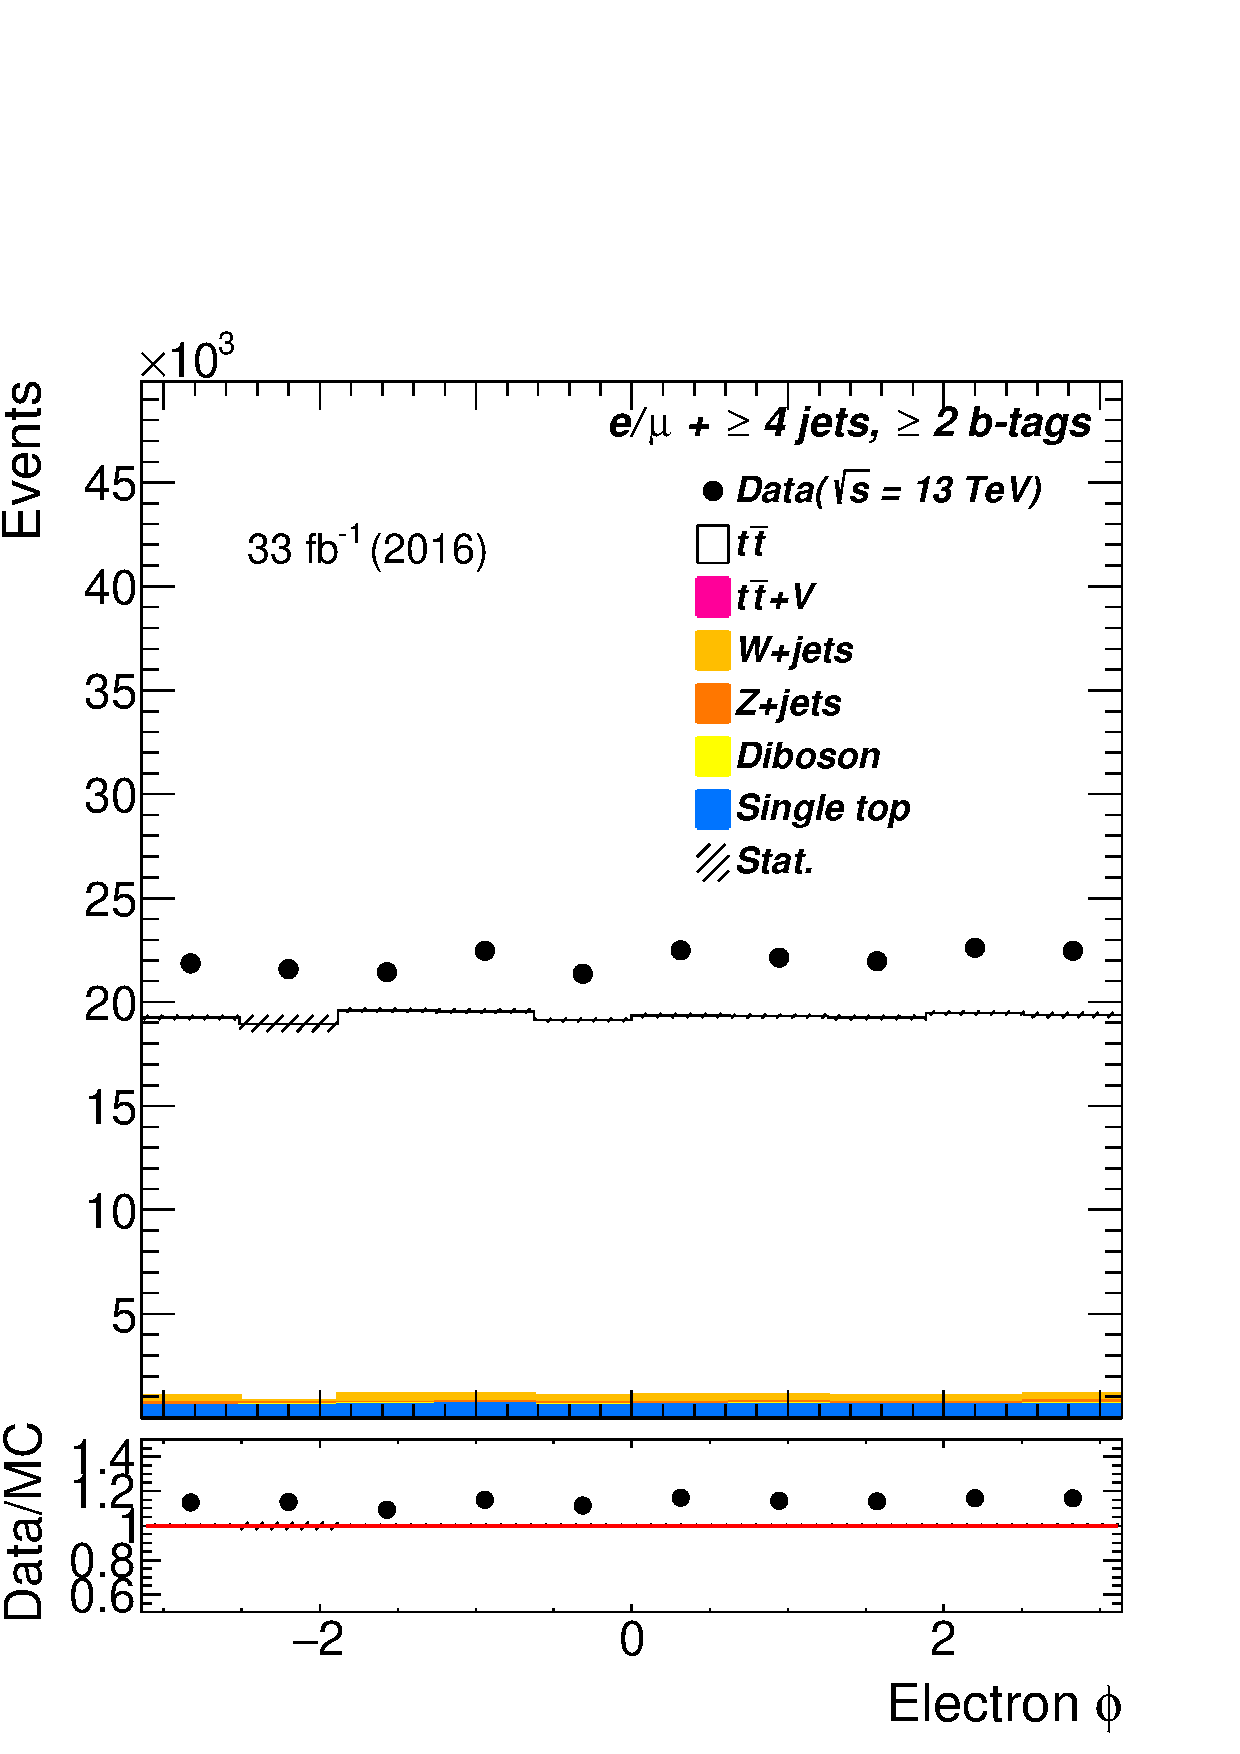
\includegraphics[width=\linewidth]{ControlPlots_emujets_2016_4incl_2incl/el_phi_emujets_2016.png}
		\caption{$\phi$ of the electrons.} \label{fig:d1}
	\end{subfigure}\hspace*{1.0cm}
\begin{subfigure}{0.25\textwidth}
	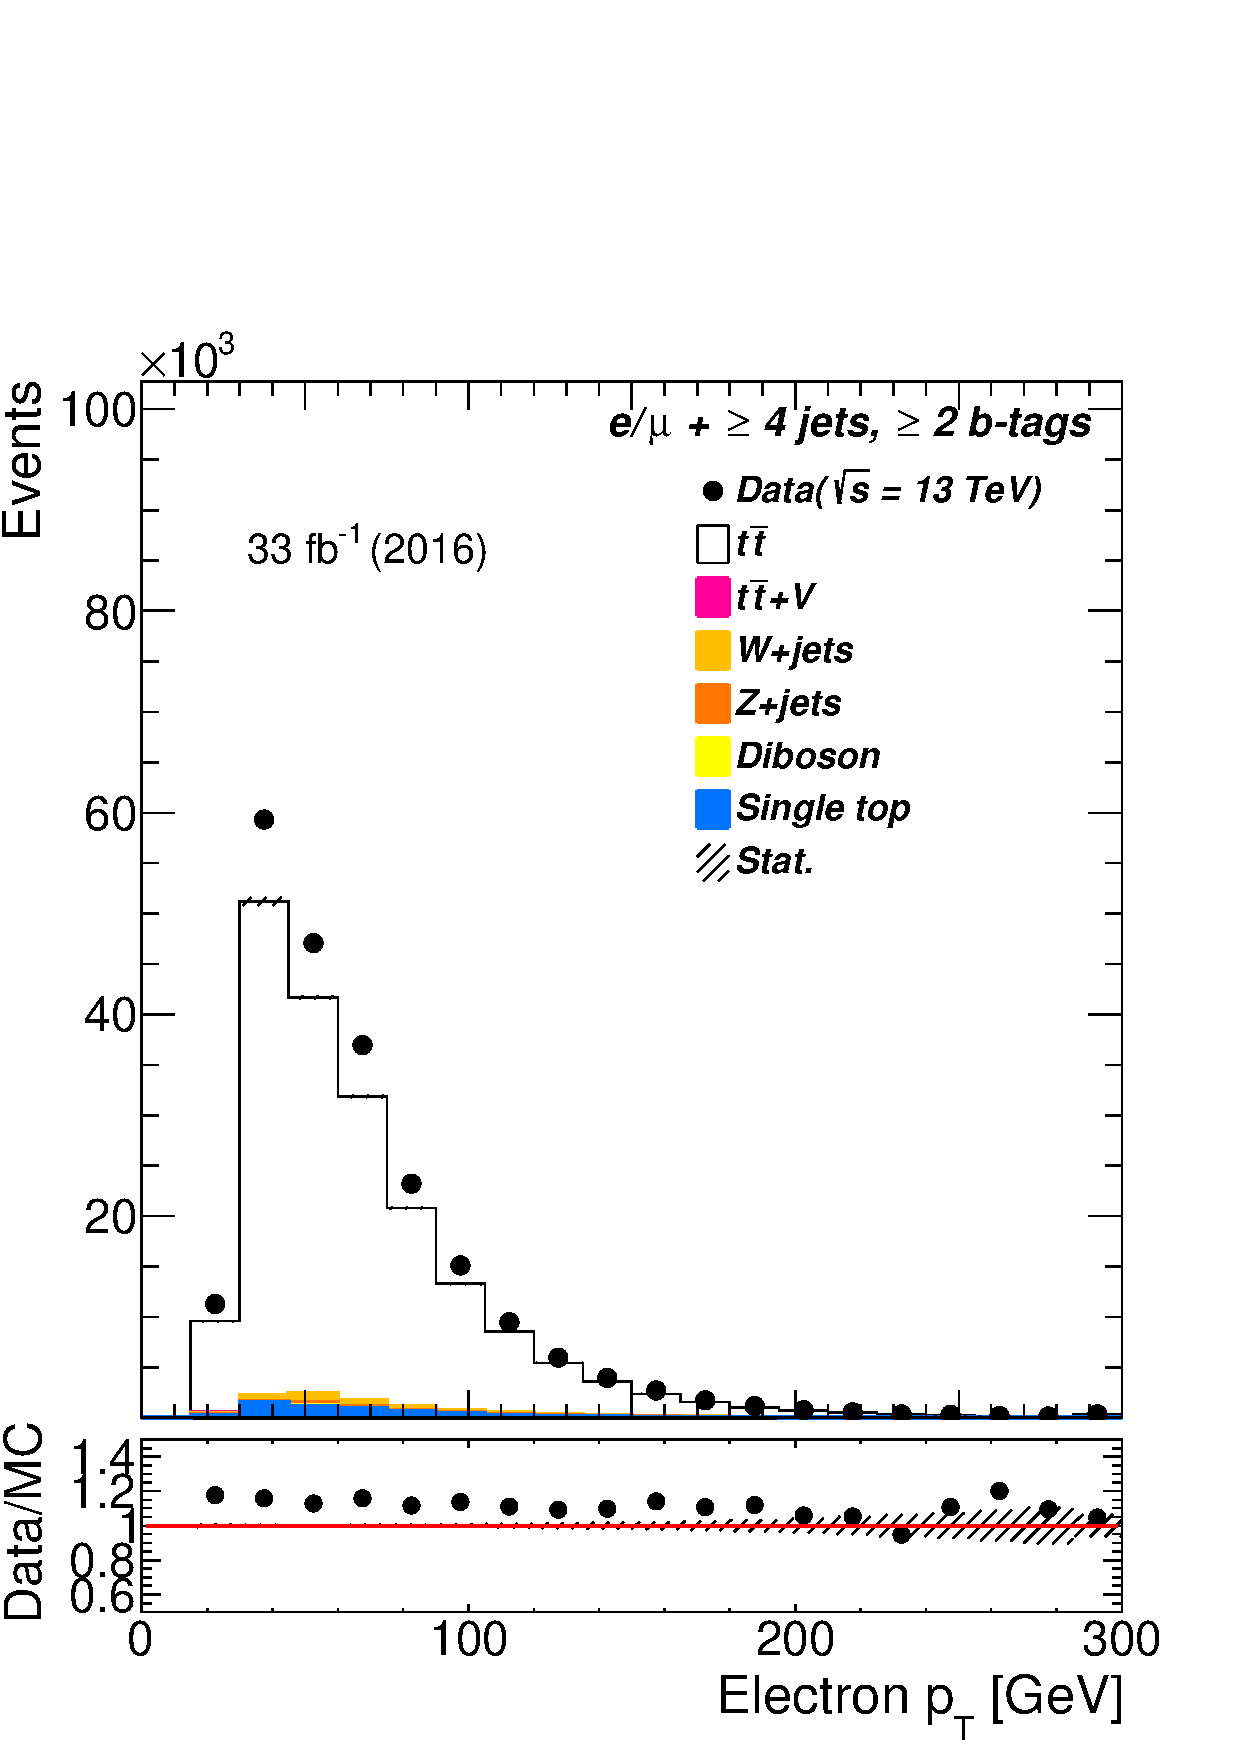
\includegraphics[width=\linewidth]{ControlPlots_emujets_2016_4incl_2incl/el_pt_emujets_2016.png}
	\caption{Transverse elec. momentum.} \label{fig:e31}
\end{subfigure}\hspace*{1.0cm}
\begin{subfigure}{0.25\textwidth}
	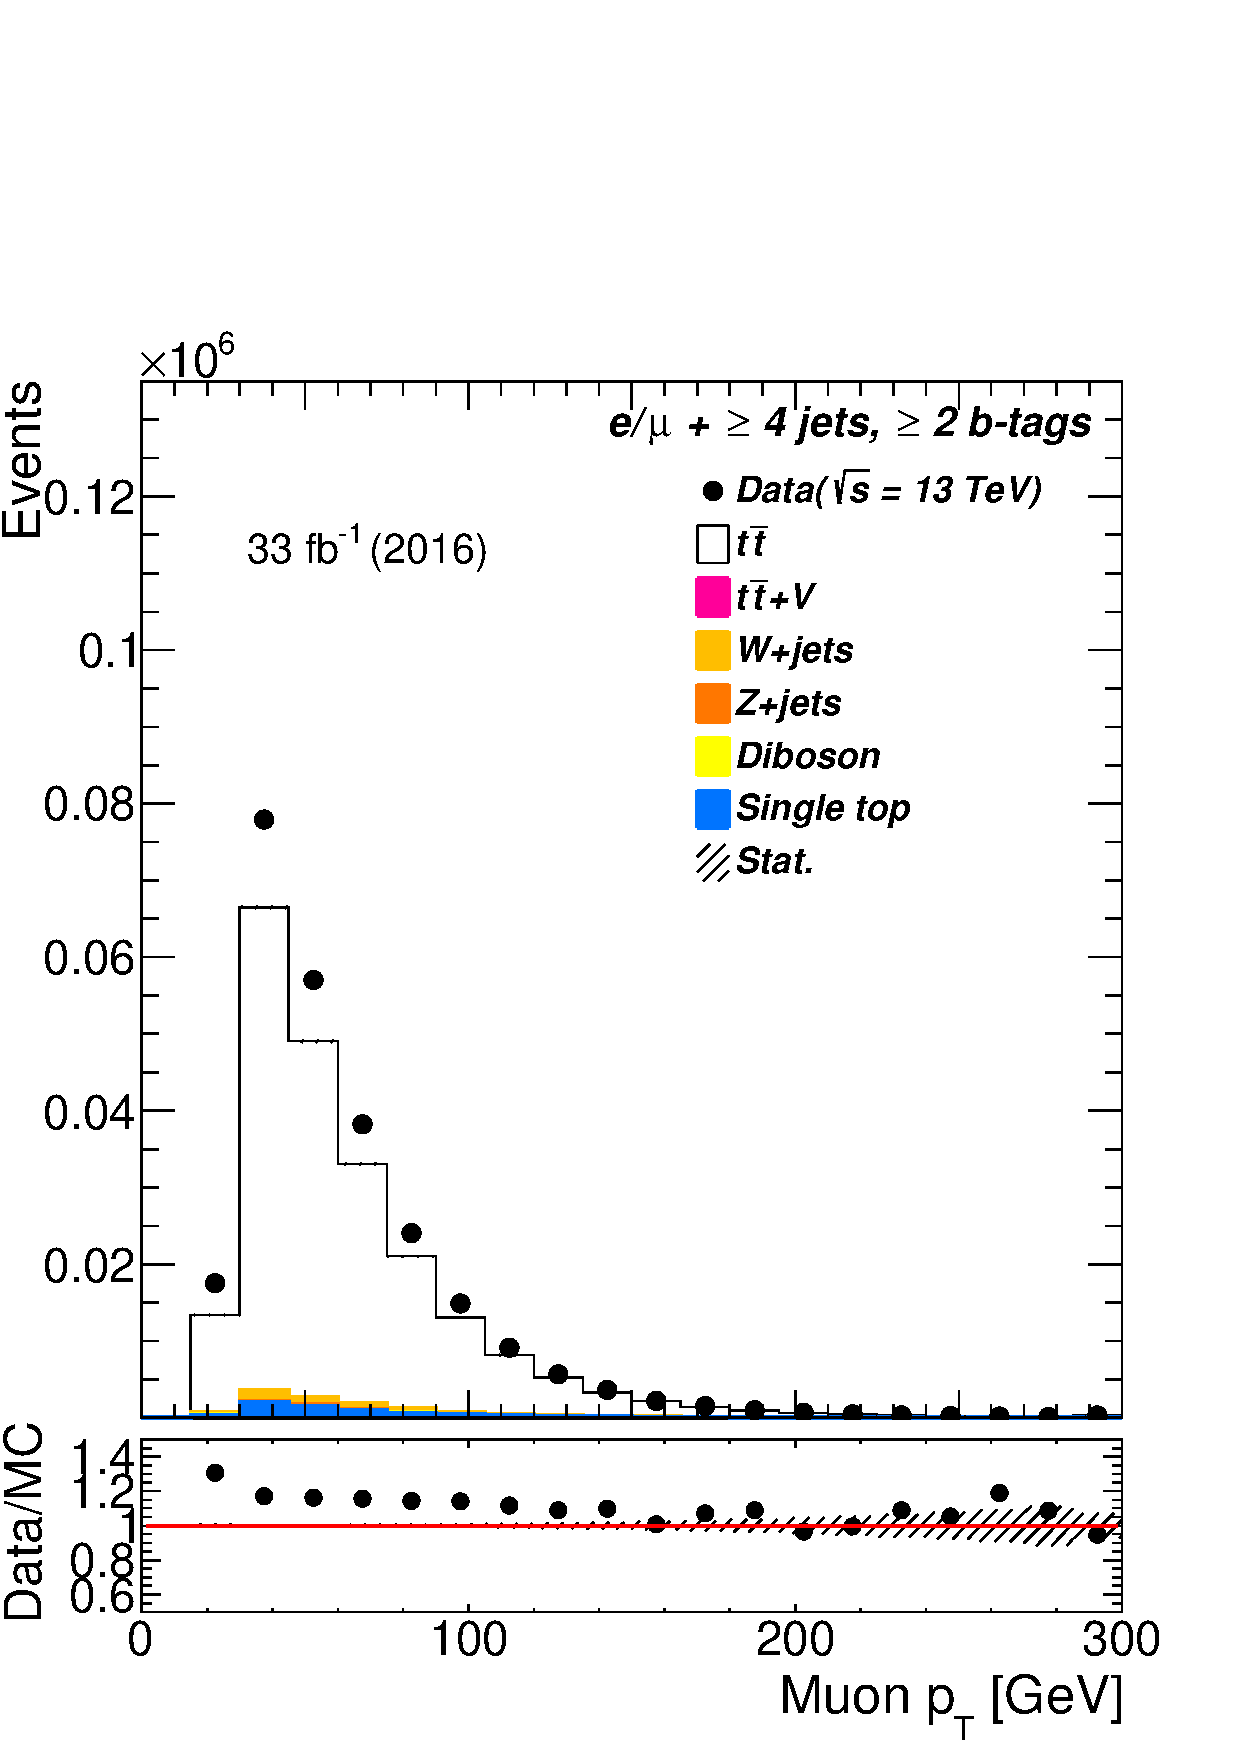
\includegraphics[width=\linewidth]{ControlPlots_emujets_2016_4incl_2incl/mu_pt_emujets_2016.png}
	\caption{Transverse muon momentum.} \label{fig:f31}
\end{subfigure}

		\caption{Global quantities for electron and muon candidates, obtained for the one $b$-tag sample.}
\end{figure}


	
	
	
	
	\begin{figure} % "[t!]" placement specifier just for this example
		\centering
	
	\medskip
	\begin{subfigure}{0.25\textwidth}
		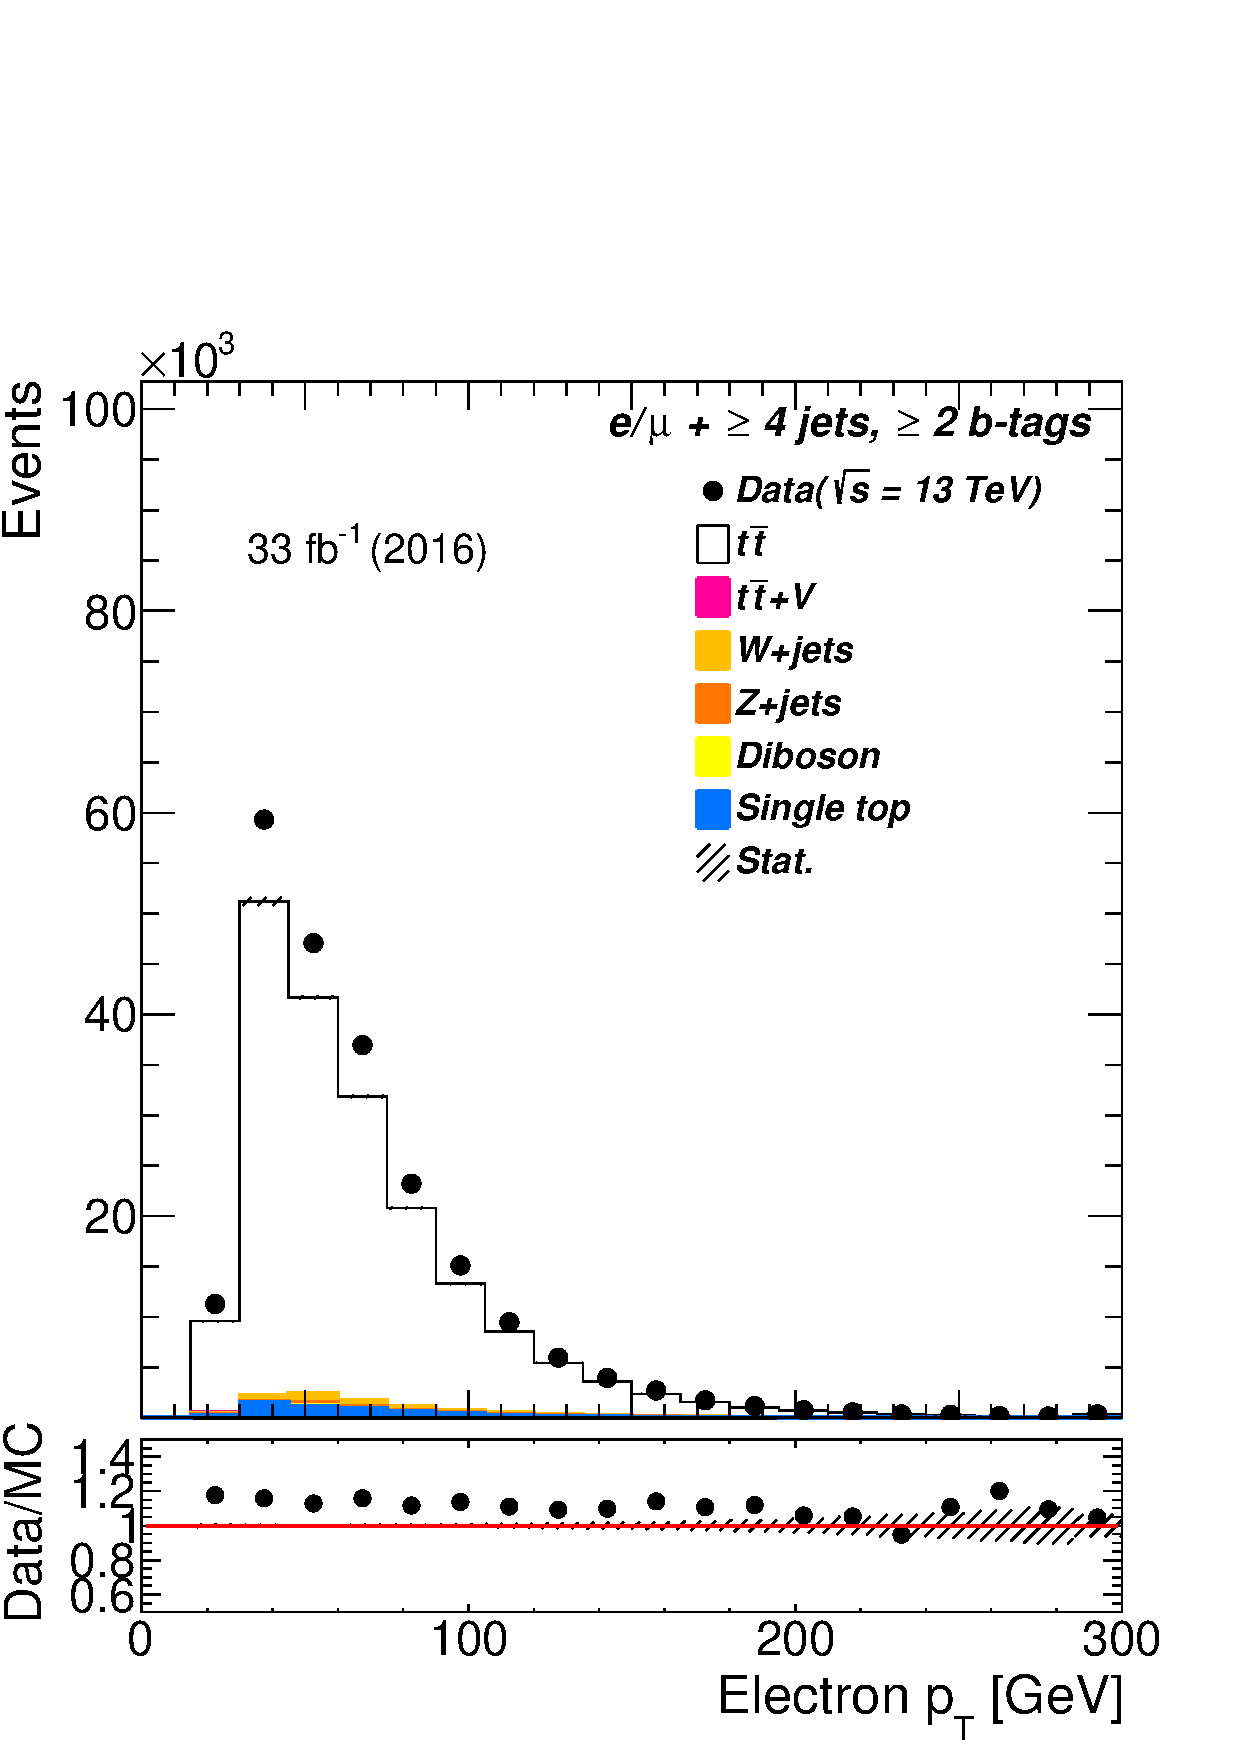
\includegraphics[width=\linewidth]{ControlPlots_emujets_2016_4incl_2incl/el_pt_emujets_2016.png}
		\caption{Transverse elec. momentum.} \label{fig:e1}
	\end{subfigure}\hspace*{1.0cm}
	\begin{subfigure}{0.25\textwidth}
		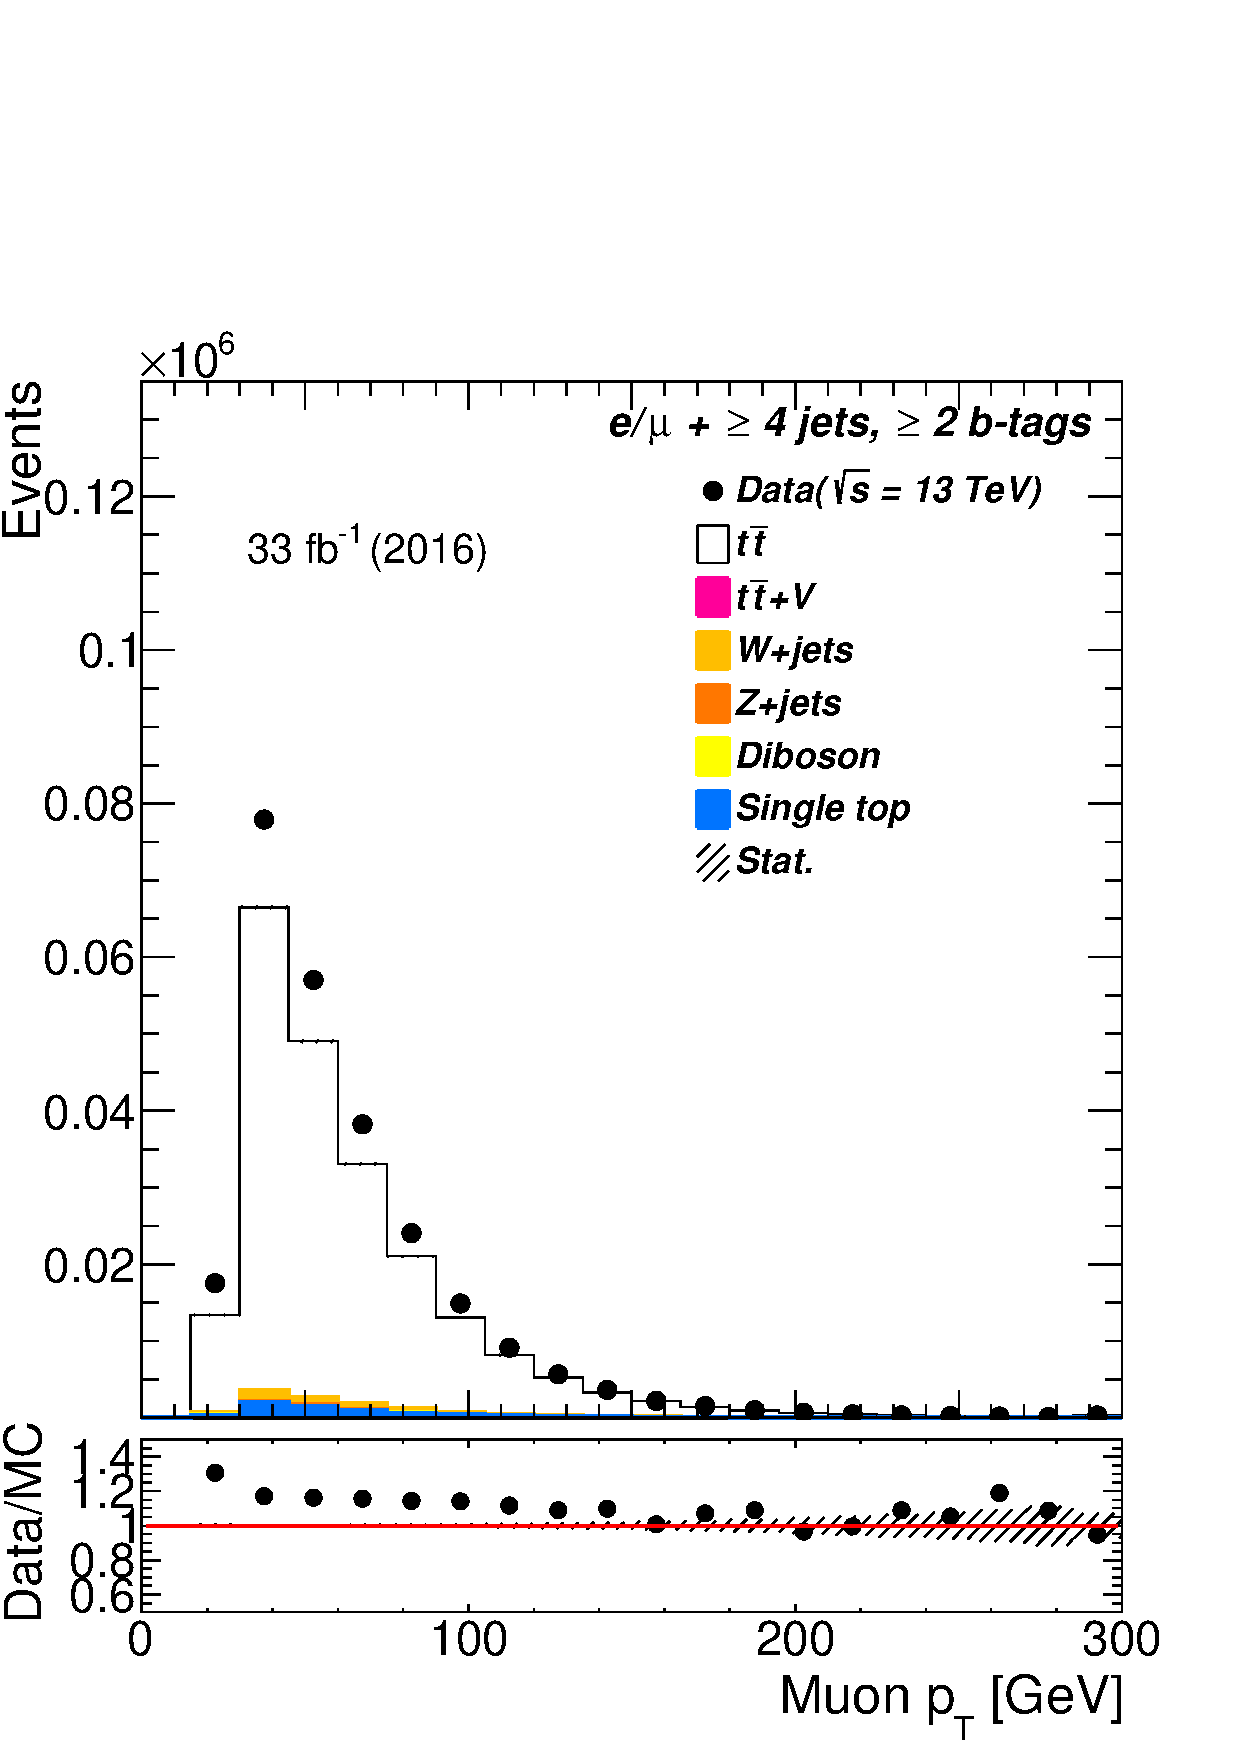
\includegraphics[width=\linewidth]{ControlPlots_emujets_2016_4incl_2incl/mu_pt_emujets_2016.png}
		\caption{Transverse muon momentum.} \label{fig:f1}
	\end{subfigure}\hspace*{1.0cm}
	\begin{subfigure}{0.25\textwidth}
		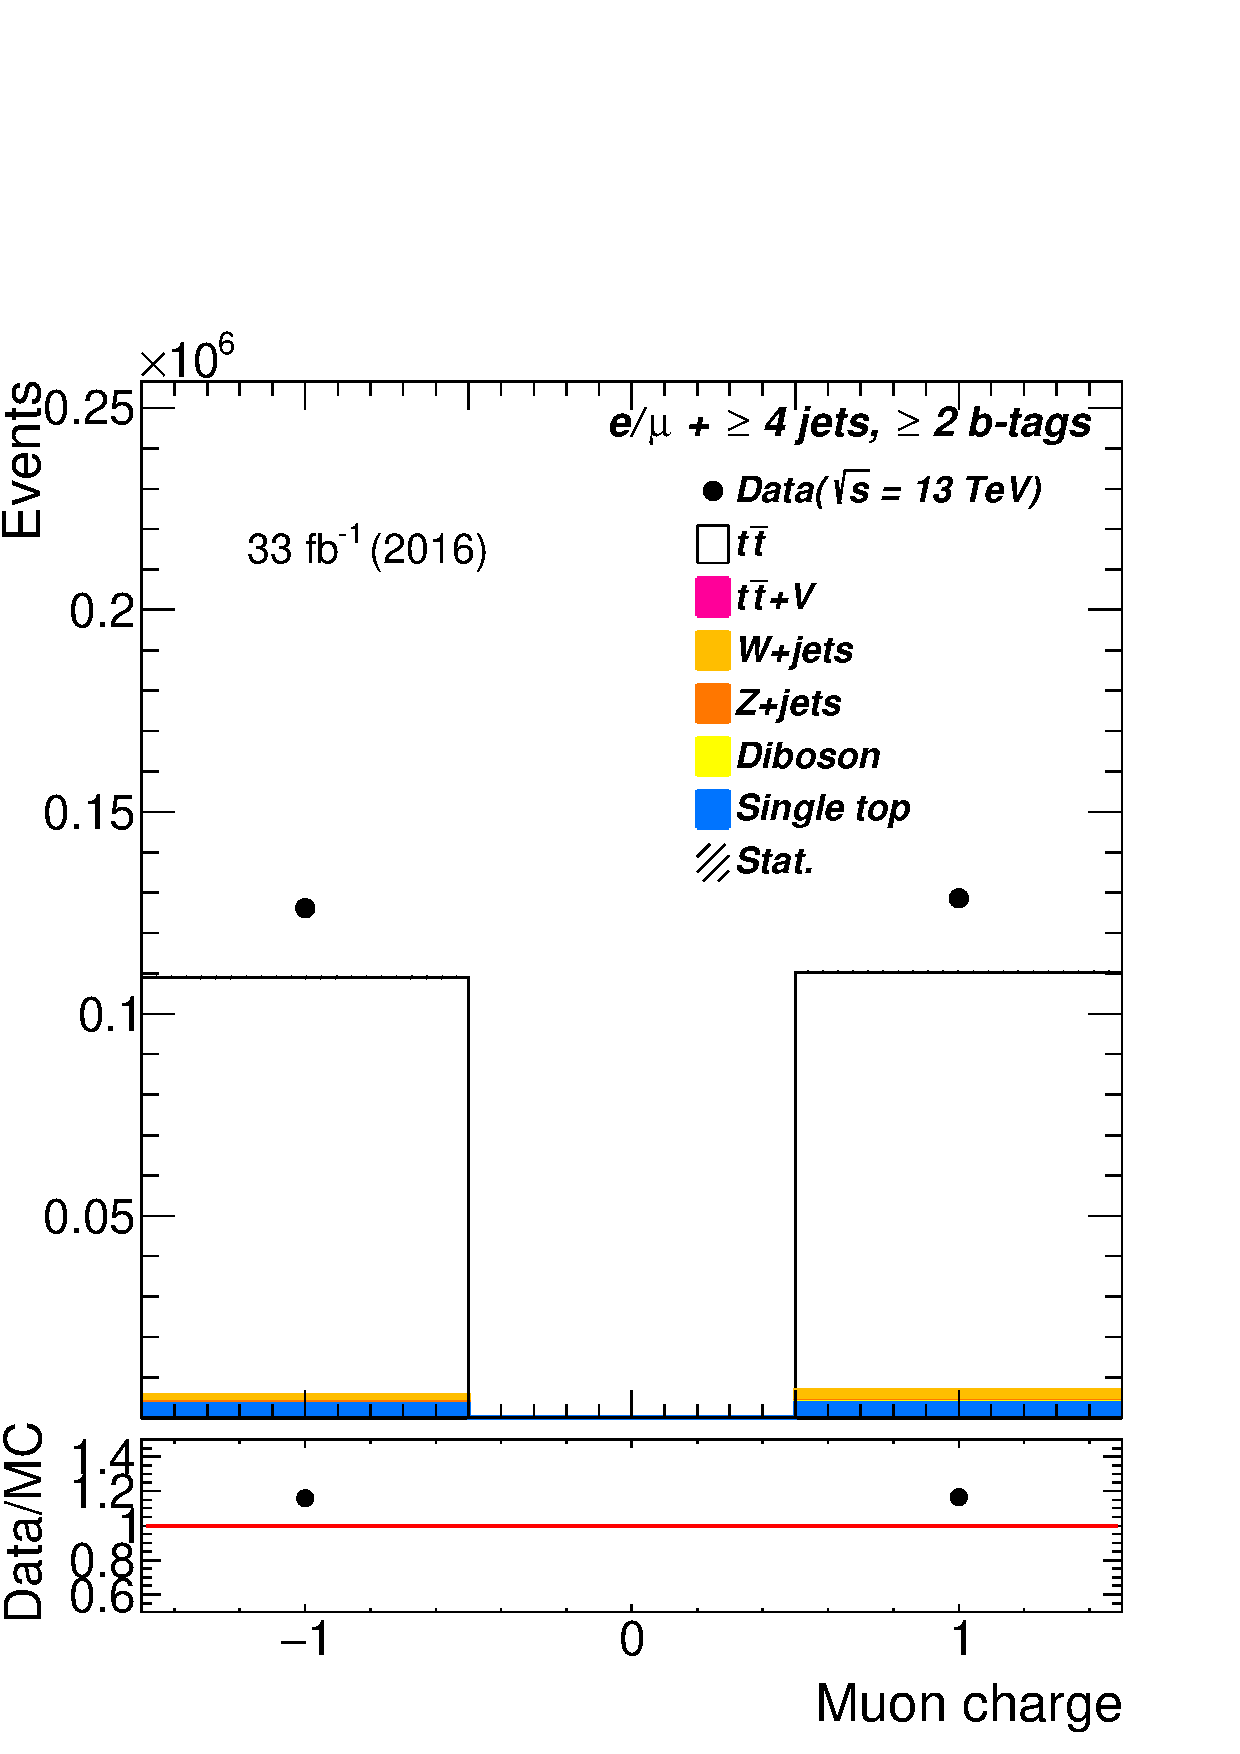
\includegraphics[width=\linewidth]{ControlPlots_emujets_2016_4incl_2incl/mu_charge_emujets_2016.png}
		\caption{Muon charge} \label{fig:a2}
	\end{subfigure}


	\begin{subfigure}{0.25\textwidth}
		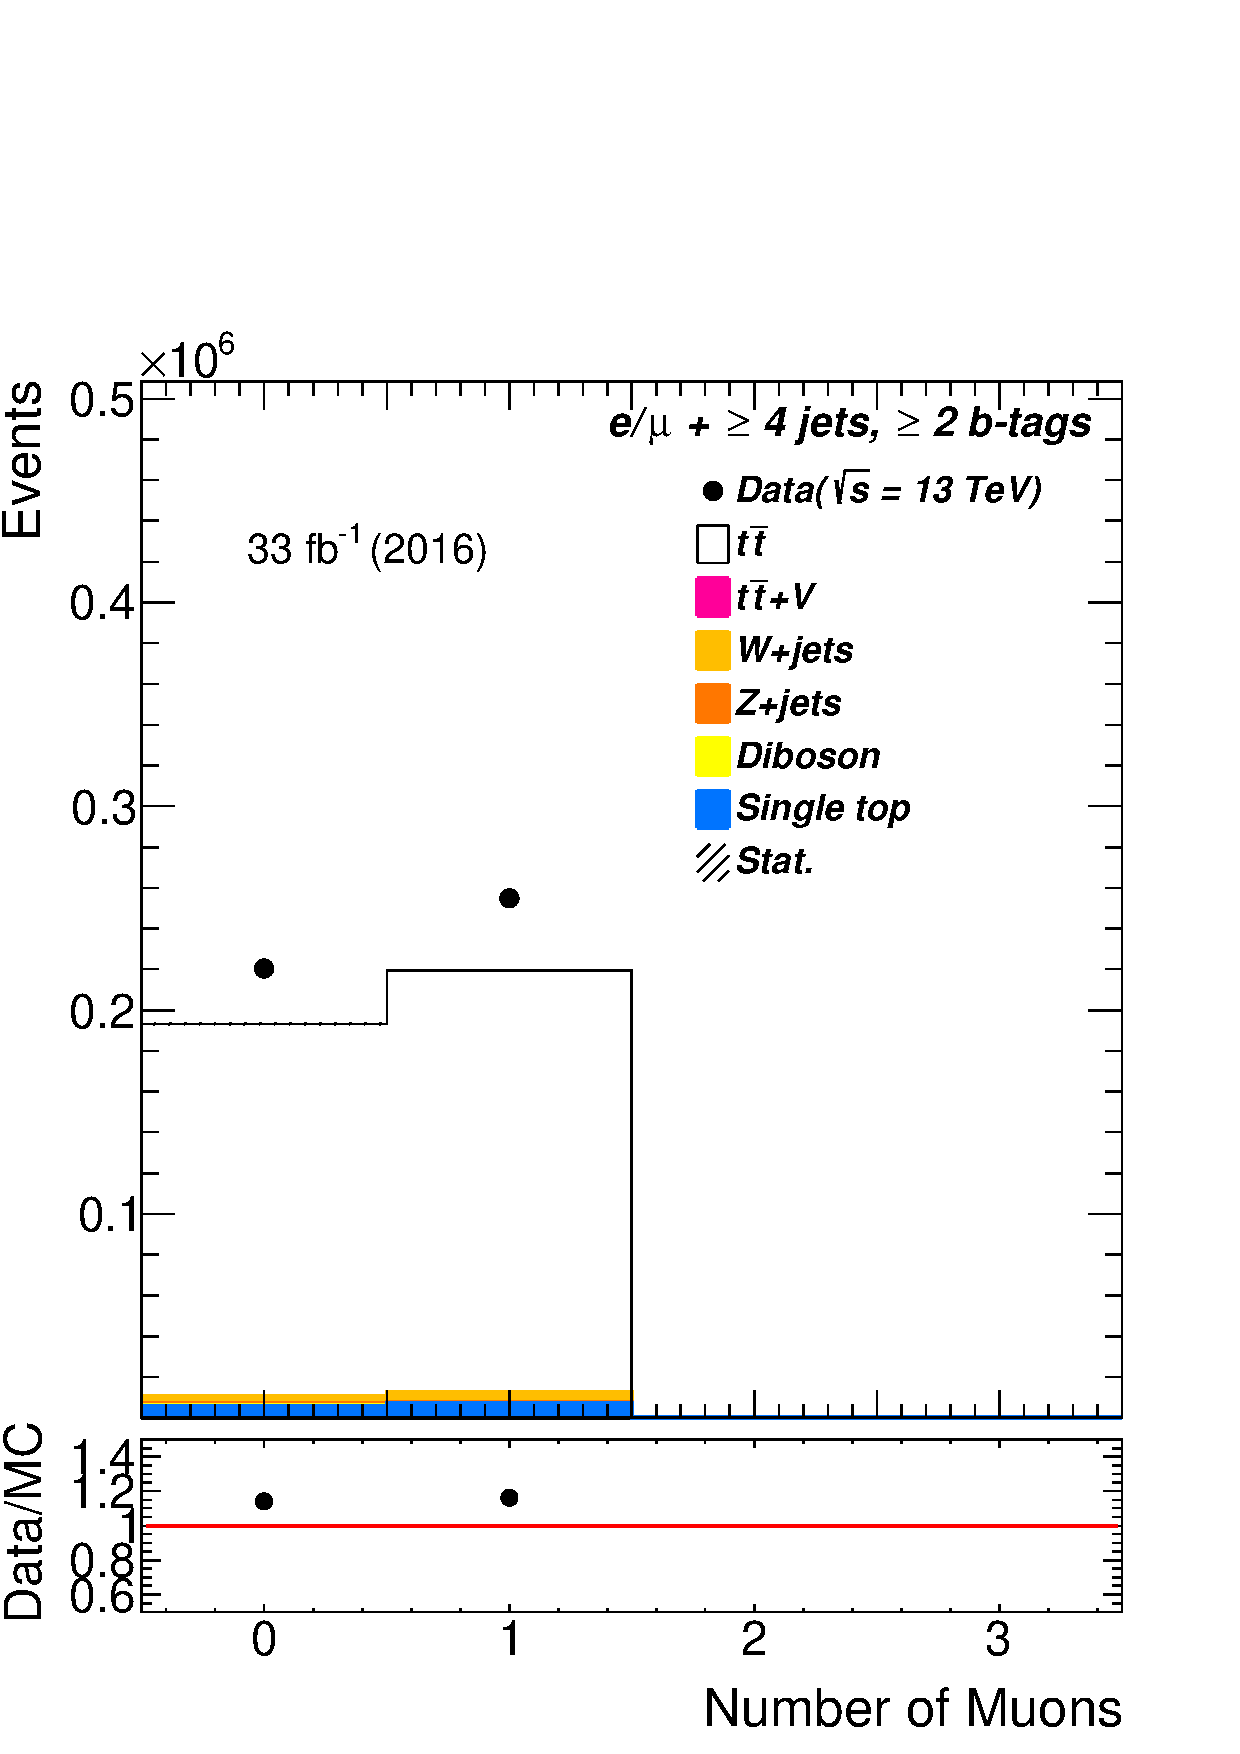
\includegraphics[width=\linewidth]{ControlPlots_emujets_2016_4incl_2incl/mu_n_emujets_2016.png}
		\caption{Number of muons.} \label{fig:b2}
	\end{subfigure}\hspace*{1.0cm}
	\begin{subfigure}{0.25\textwidth}
		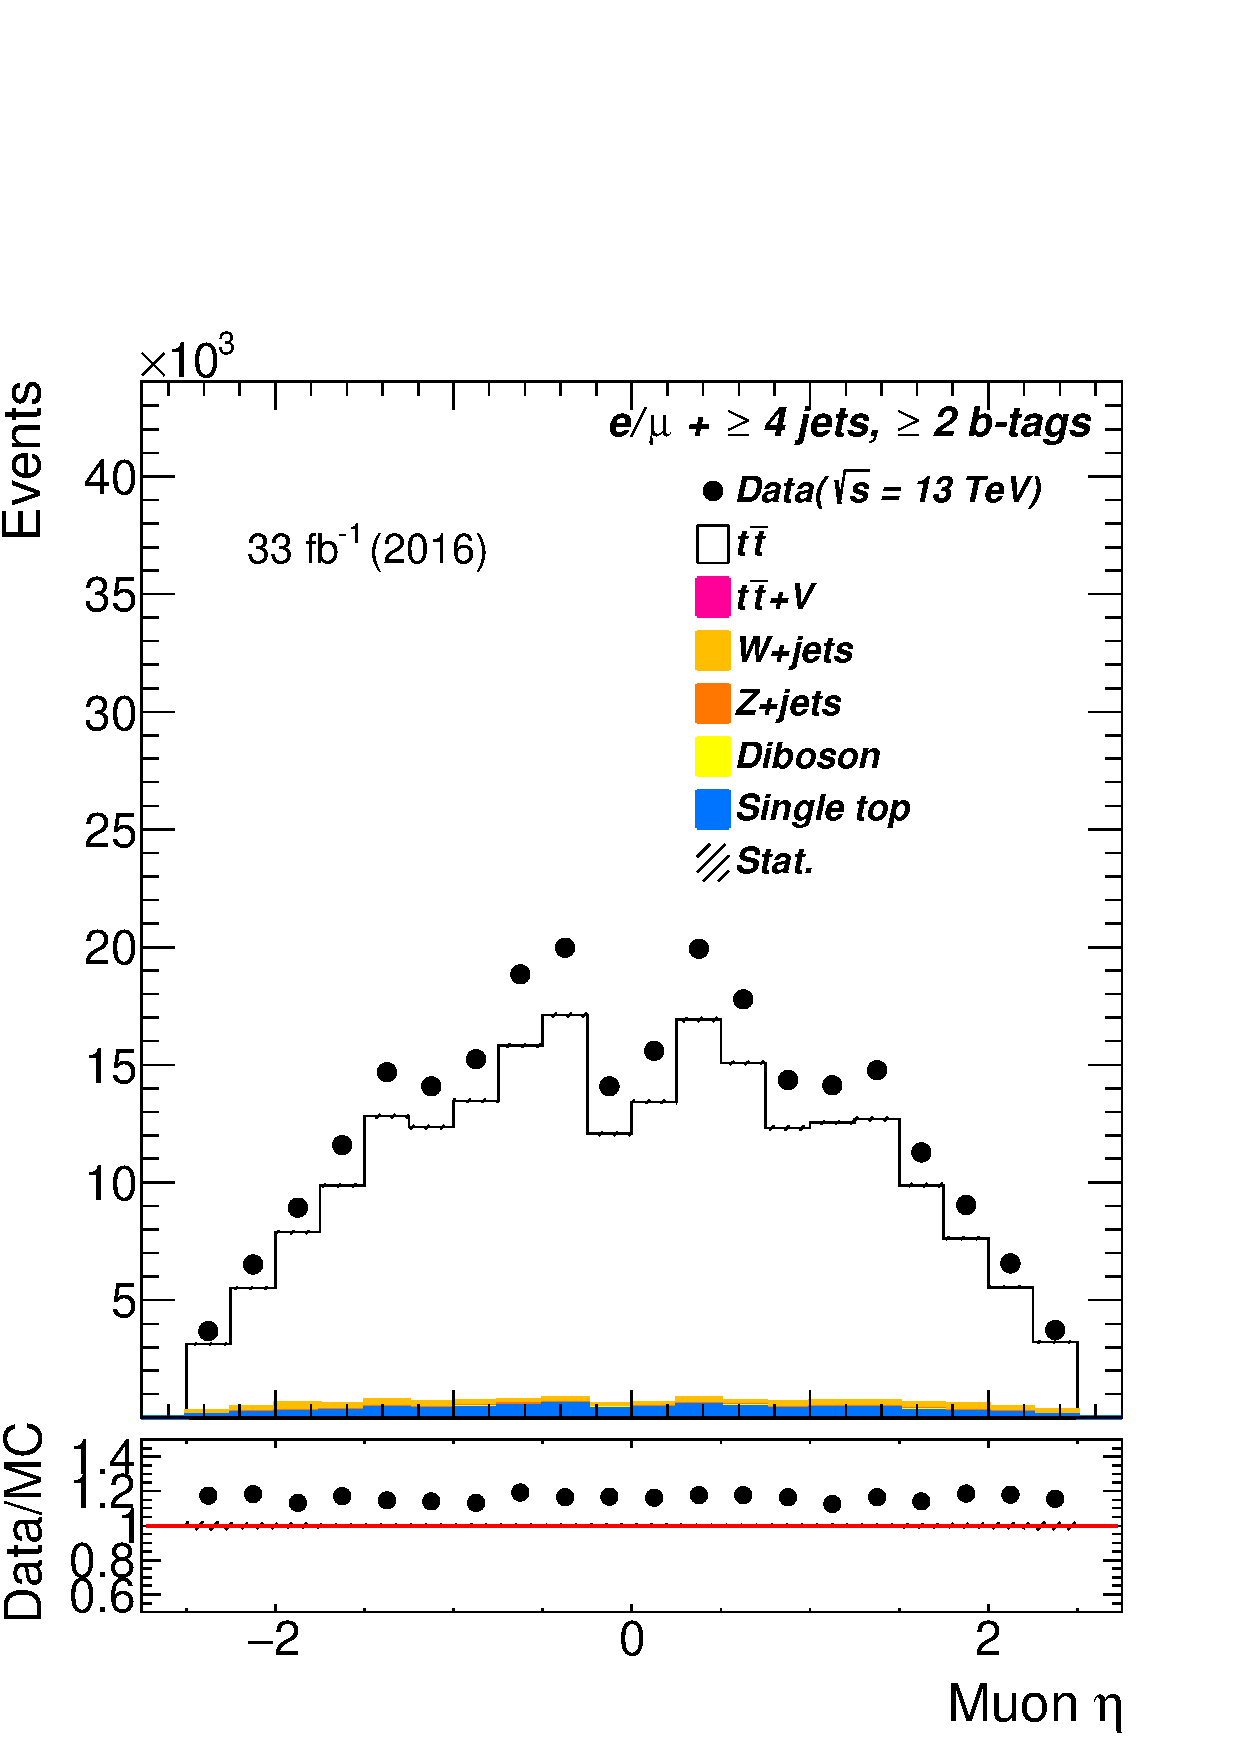
\includegraphics[width=\linewidth]{ControlPlots_emujets_2016_4incl_2incl/mu_eta_emujets_2016.png}
		\caption{Rapidity the muons} \label{fig:c2}
	\end{subfigure}\hspace*{1.0cm}
	\begin{subfigure}{0.25\textwidth}
		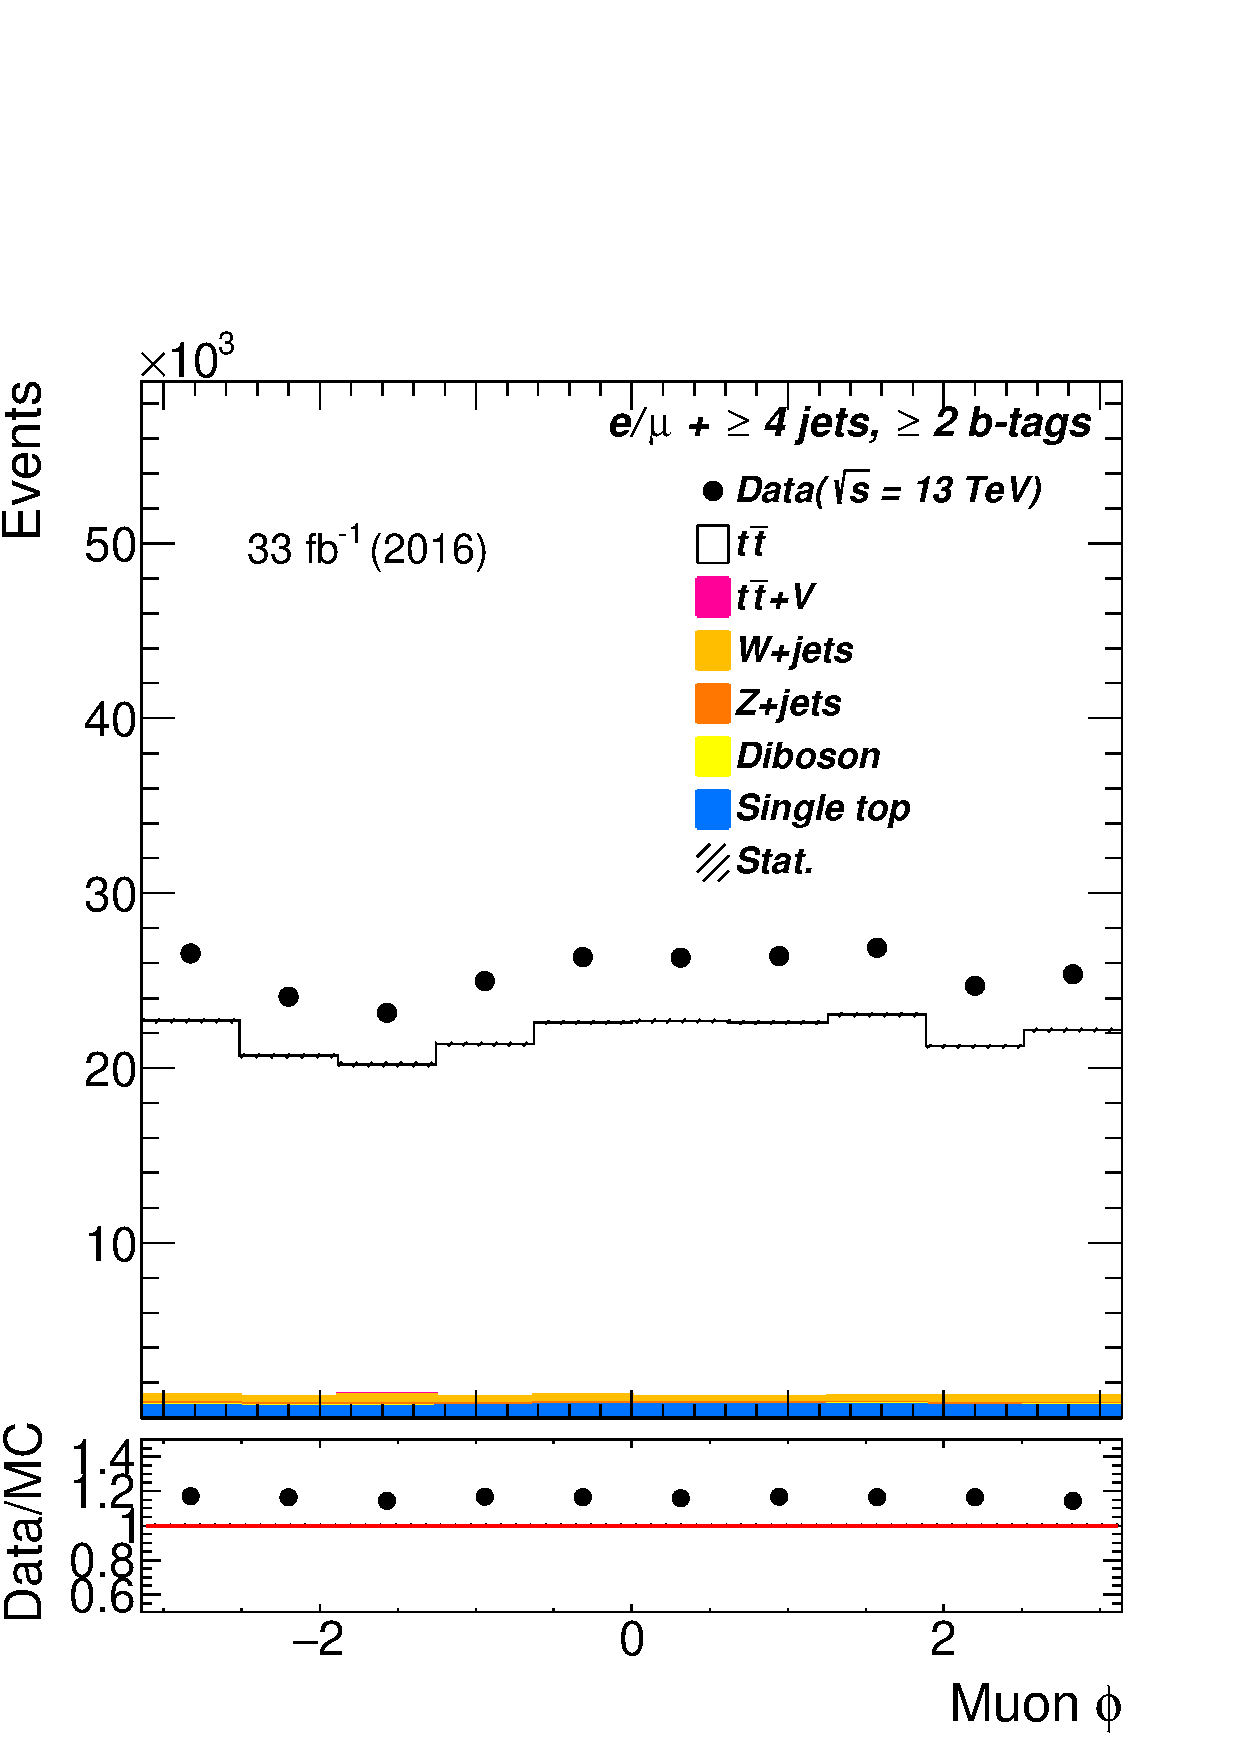
\includegraphics[width=\linewidth]{ControlPlots_emujets_2016_4incl_2incl/mu_phi_emujets_2016.png}
		\caption{$\Phi$ of the muons.} \label{fig:d2}
	\end{subfigure}


	\begin{subfigure}{0.25\textwidth}
	\includegraphics[width=\linewidth]{ControlPlots_emujets_2016_4incl_2incl/jet0_eta_emujets_2016.png}
	\caption{Rapidity  the first jet.} \label{fig:e2}
   \end{subfigure}\hspace*{1.0cm}
  \begin{subfigure}{0.25\textwidth}
	\includegraphics[width=\linewidth]{ControlPlots_emujets_2016_4incl_2incl/jet0_phi_emujets_2016.png}
	\caption{$\phi$ of the first Jet.} \label{fig:f2}
\end{subfigure}\hspace*{1.0cm}
\begin{subfigure}{0.25\textwidth}
	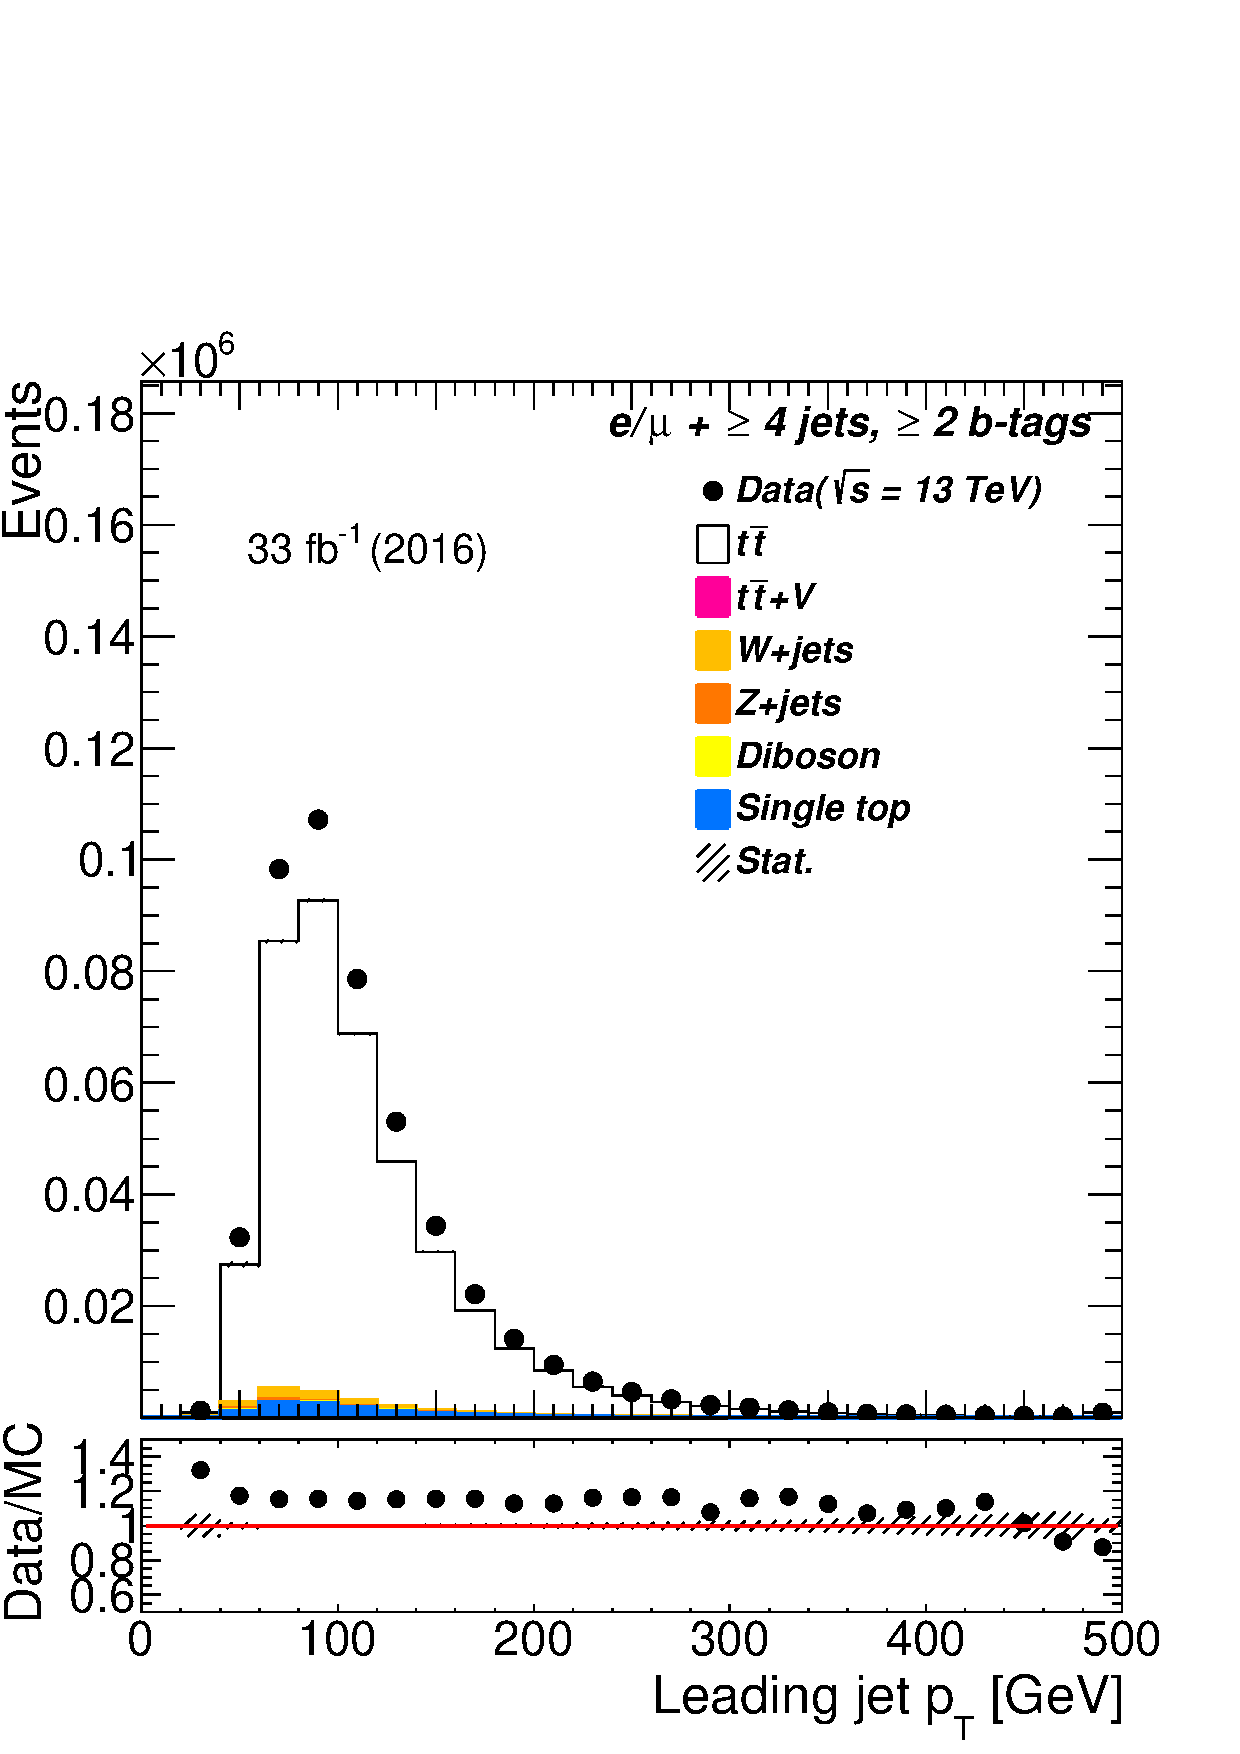
\includegraphics[width=\linewidth]{ControlPlots_emujets_2016_4incl_2incl/jet0_pt_emujets_2016.png}
	\caption{Transverse momentum of the first jet.} \label{fig:a3}
\end{subfigure}

		\caption{Global quantities  muon candidates, as well for the first and second jet, obtained for the one $b$-tag sample.}
\end{figure}





\begin{figure} % "[t!]" placement specifier just for this example
	\centering

\begin{subfigure}{0.25\textwidth}
	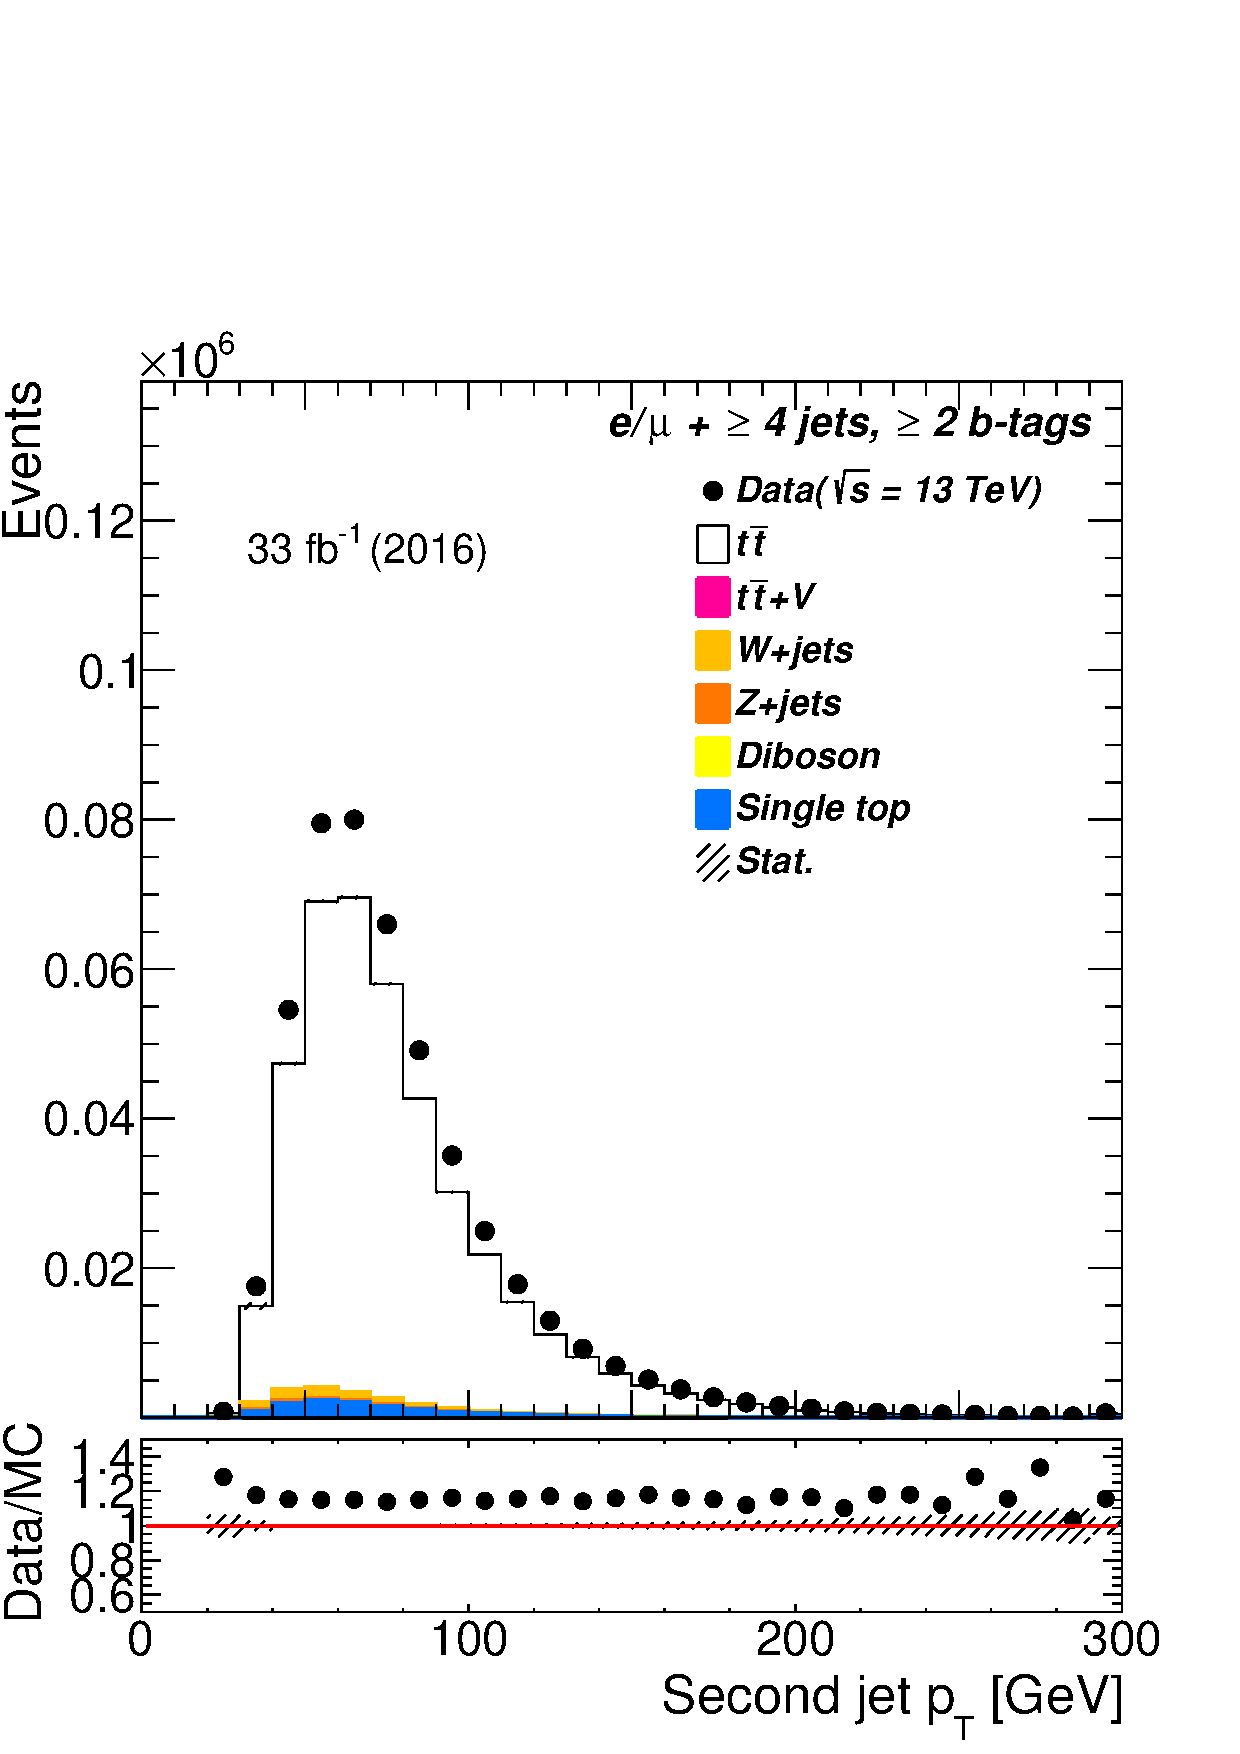
\includegraphics[width=\linewidth]{ControlPlots_emujets_2016_4incl_2incl/jet1_pt_emujets_2016.png}
	\caption{Transverse momentum of the second jet.} \label{fig:b3}
\end{subfigure}\hspace*{1.0cm}
\begin{subfigure}{0.25\textwidth}
	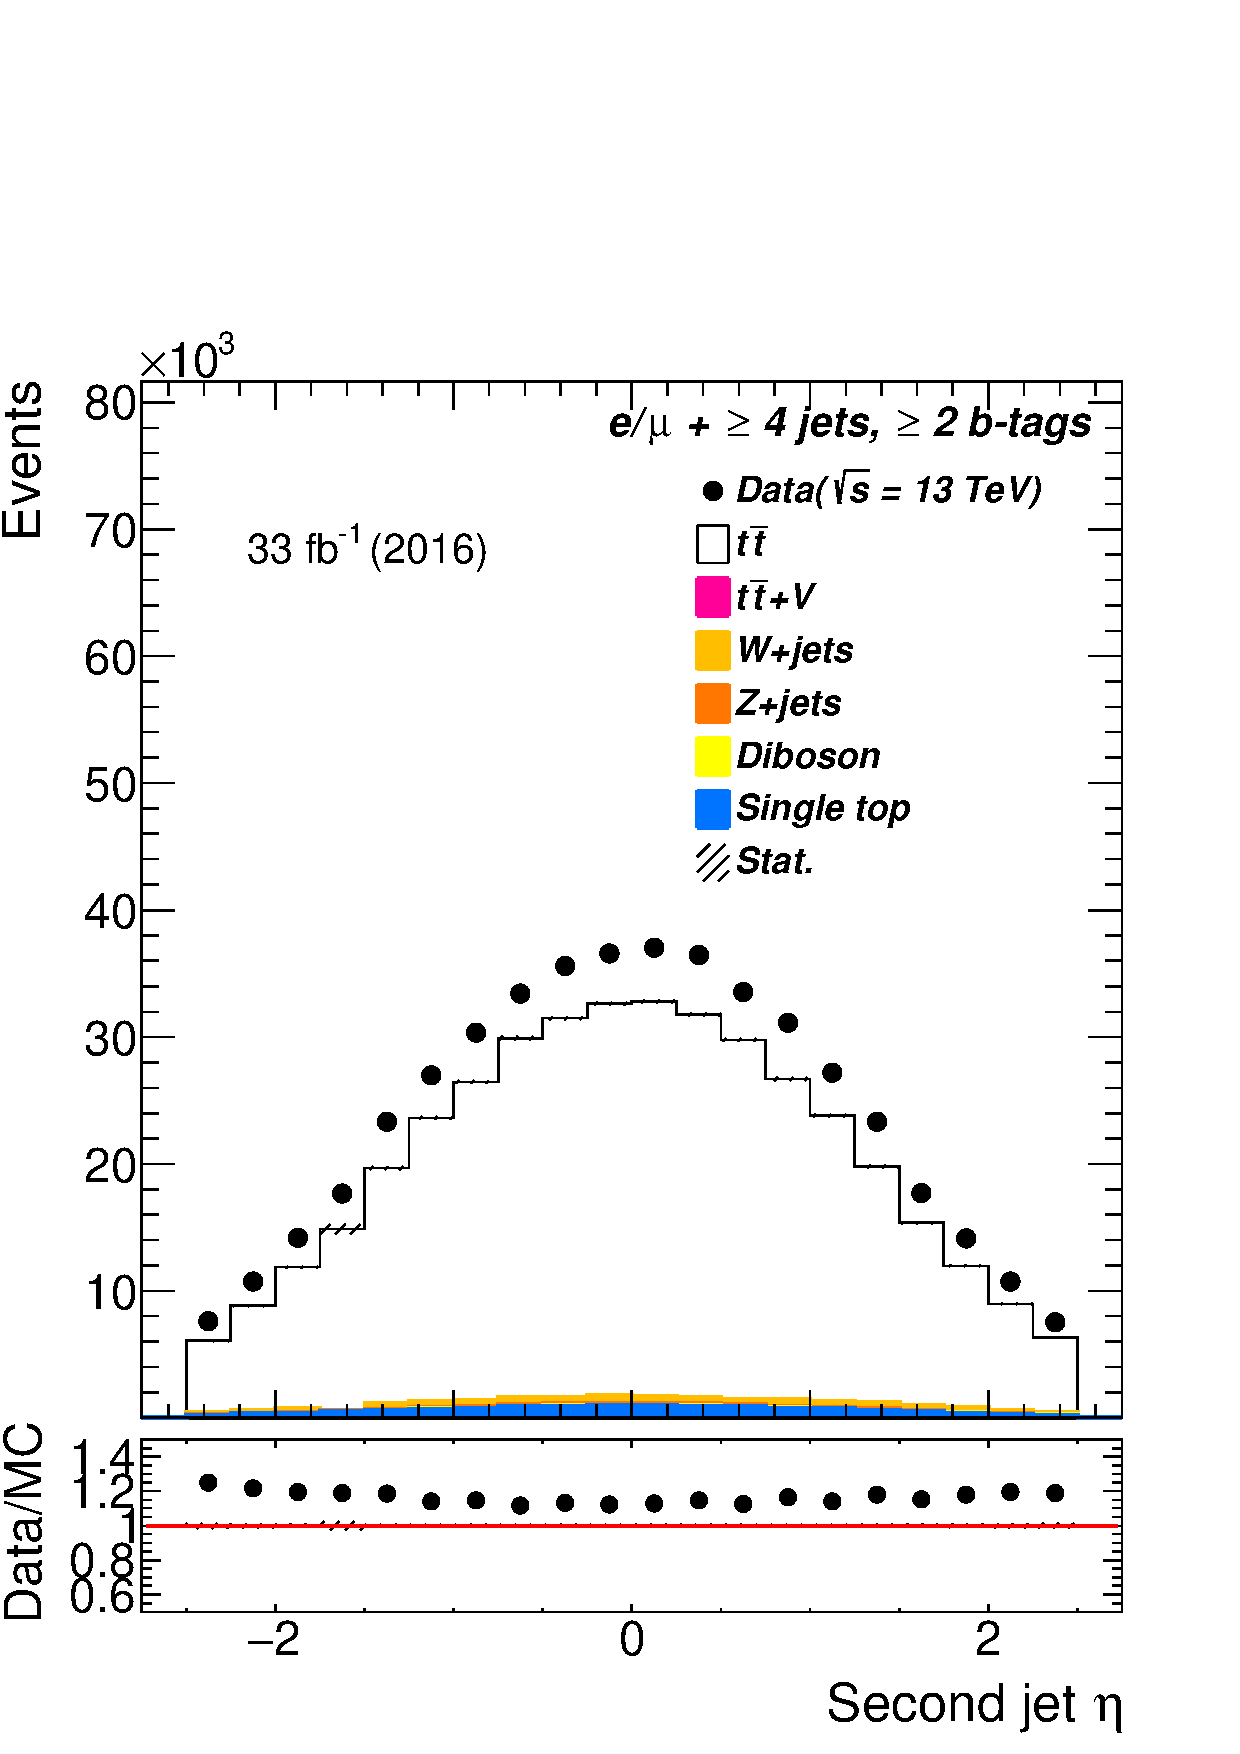
\includegraphics[width=\linewidth]{ControlPlots_emujets_2016_4incl_2incl/jet1_eta_emujets_2016.png}
	\caption{Rapidity of the second jet.} \label{fig:c3}
\end{subfigure}\hspace*{1.0cm}
\begin{subfigure}{0.25\textwidth}
	\includegraphics[width=\linewidth]{ControlPlots_emujets_2016_4incl_2incl/jet1_phi_emujets_2016.png}
	\caption{$\phi$ of the second jet.} \label{fig:d3}
\end{subfigure}




	\begin{subfigure}{0.25\textwidth}
		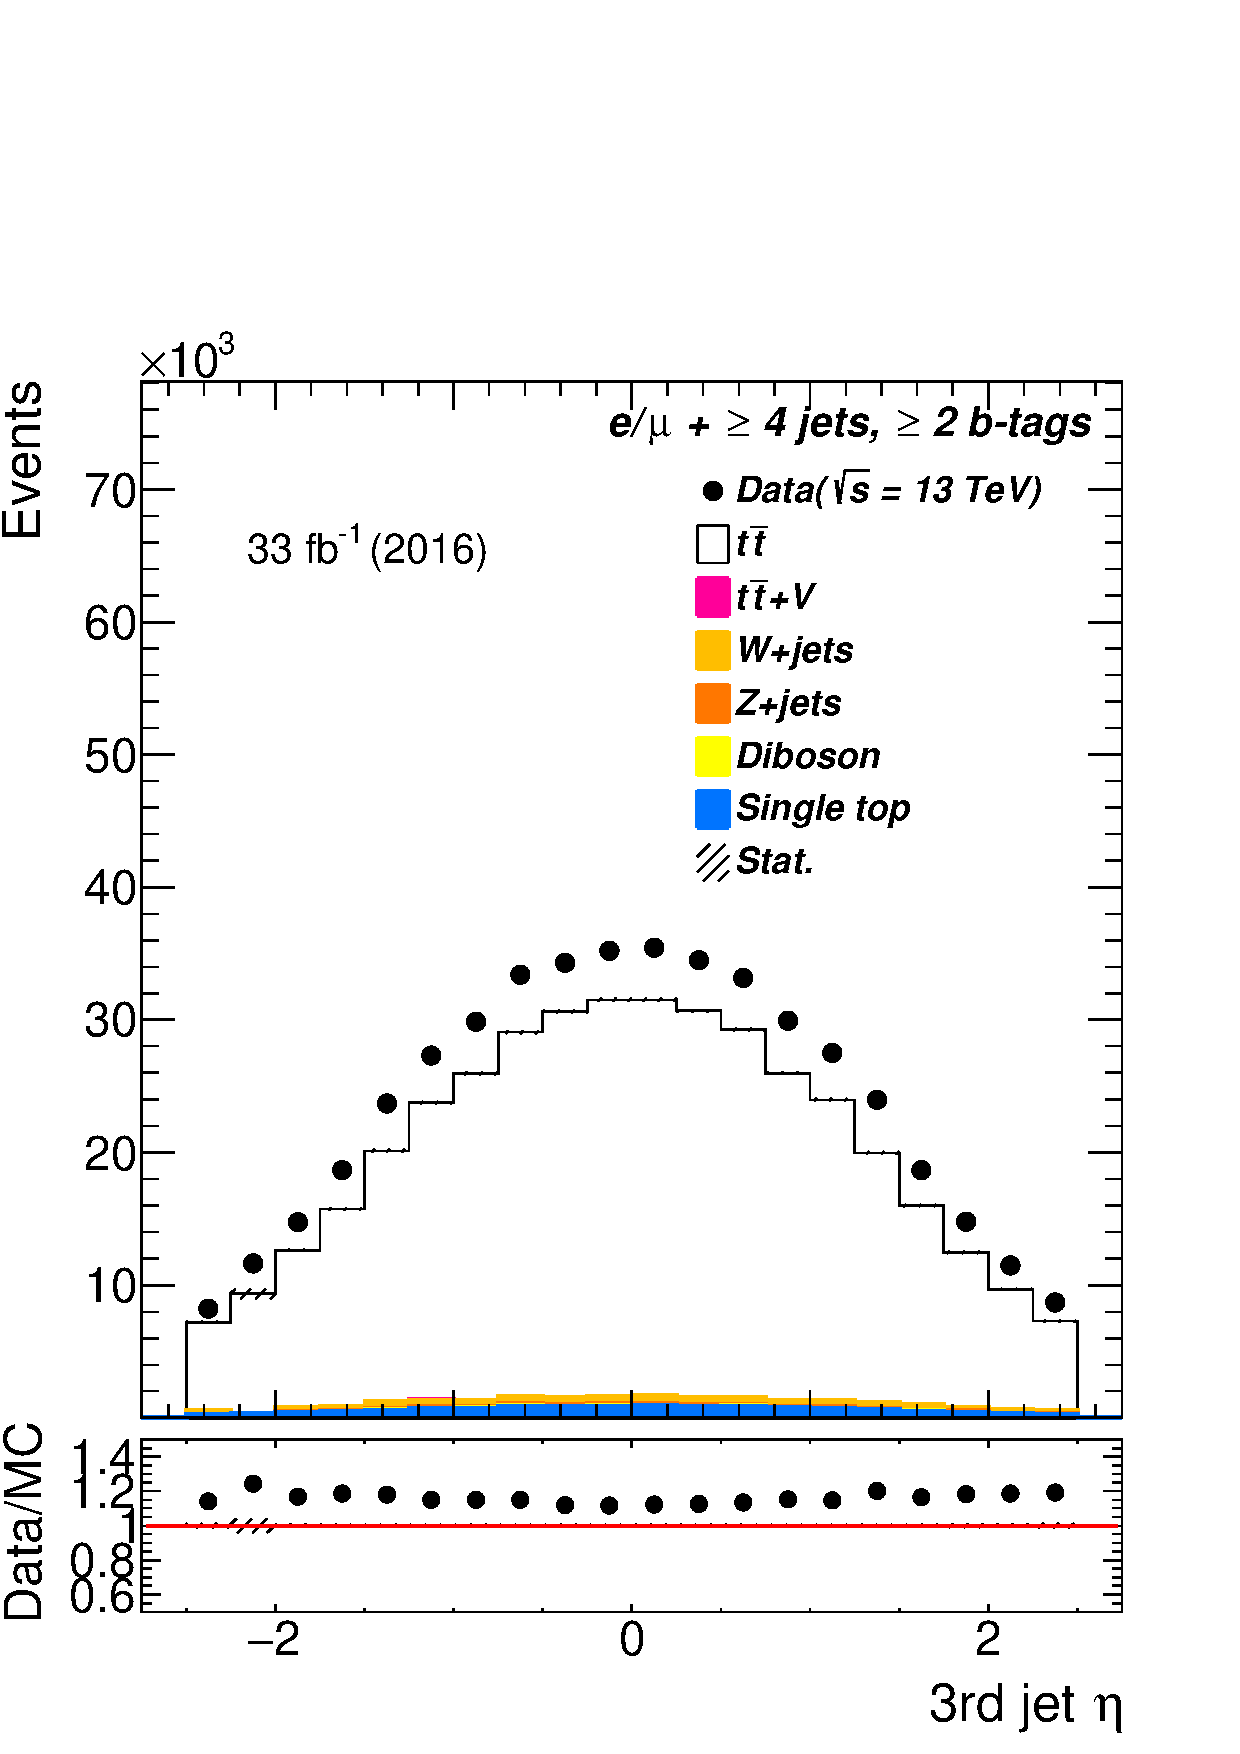
\includegraphics[width=\linewidth]{ControlPlots_emujets_2016_4incl_2incl/jet2_eta_emujets_2016.png}
		\caption{Rapidity of the third jet.} \label{fig:e3}
	\end{subfigure}\hspace*{1.0cm}
	\begin{subfigure}{0.25\textwidth}
		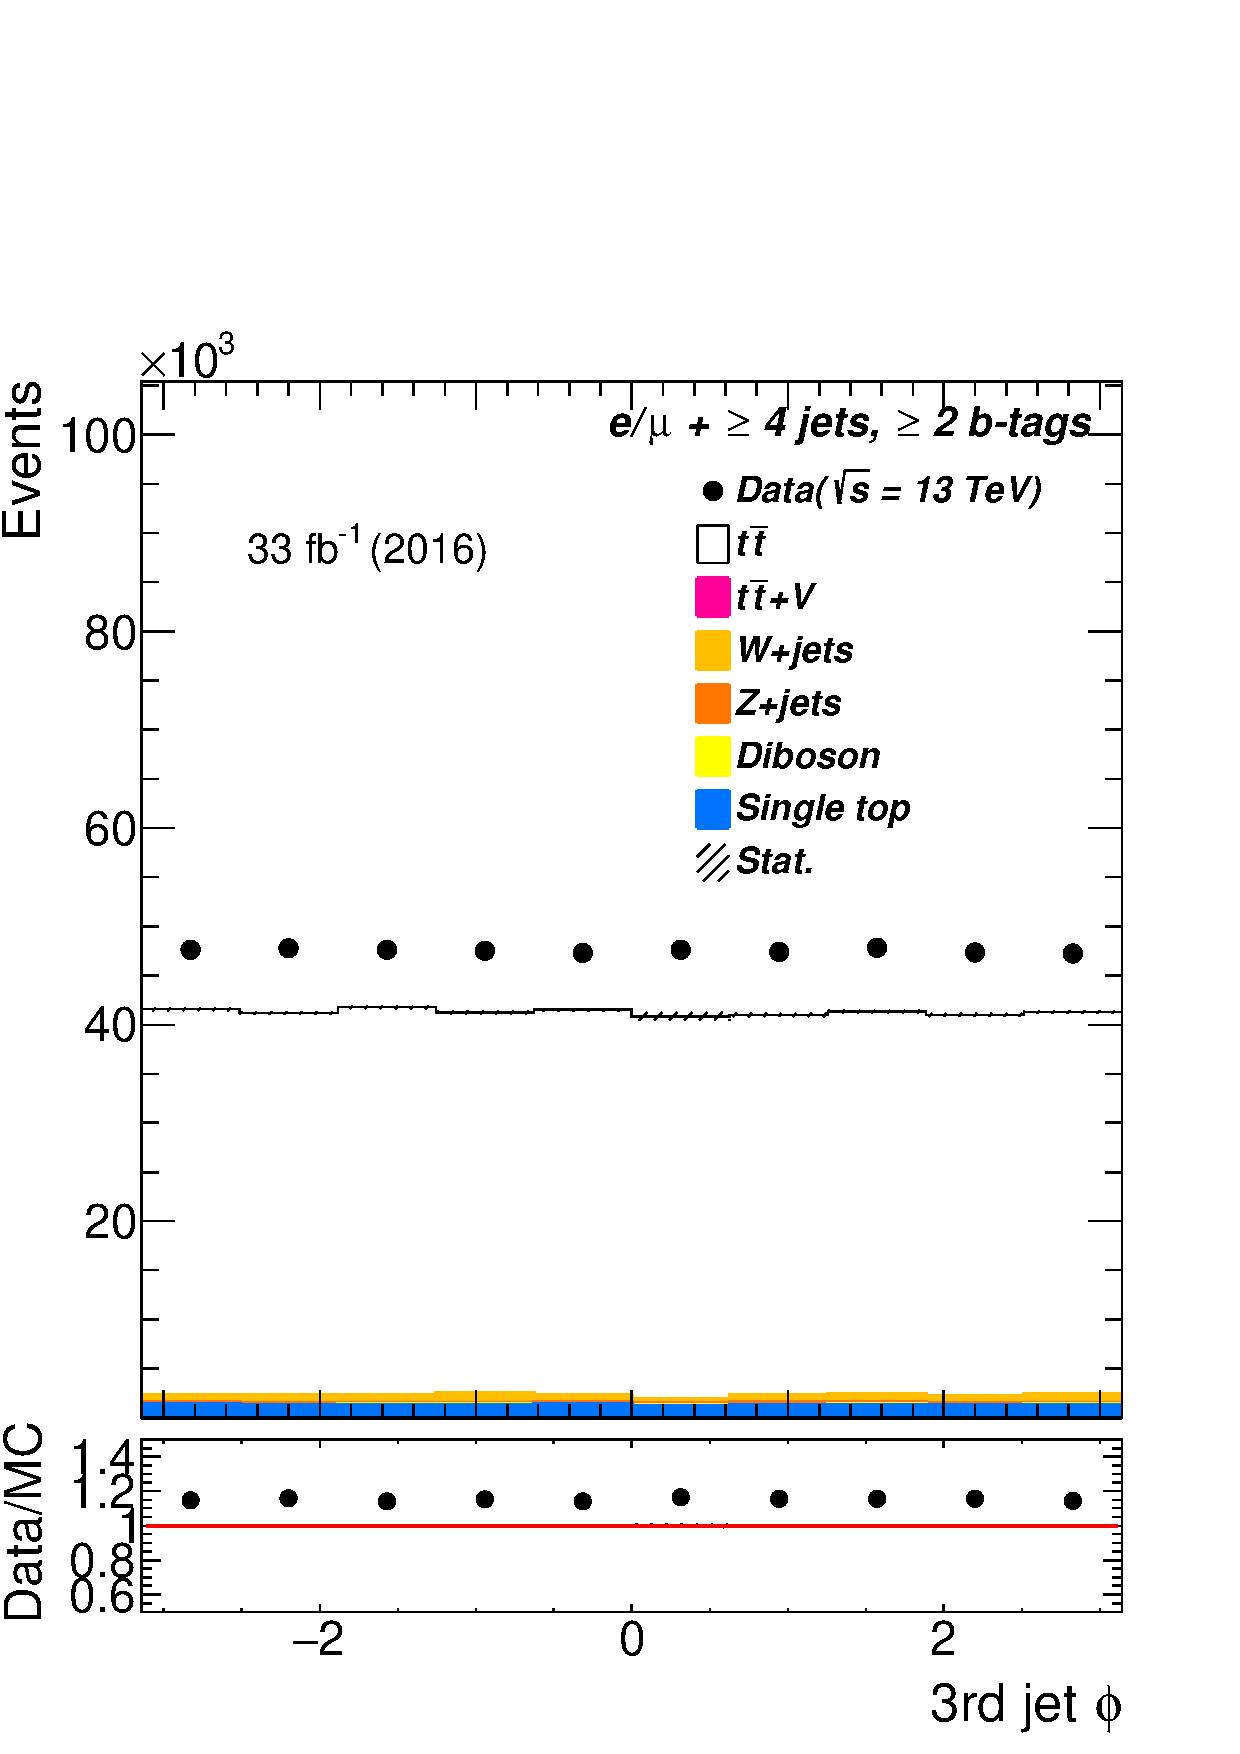
\includegraphics[width=\linewidth]{ControlPlots_emujets_2016_4incl_2incl/jet2_phi_emujets_2016.png}
		\caption{$\phi$  of the third jet.} \label{fig:f3}
	\end{subfigure}\hspace*{1.0cm}
	\begin{subfigure}{0.25\textwidth}
	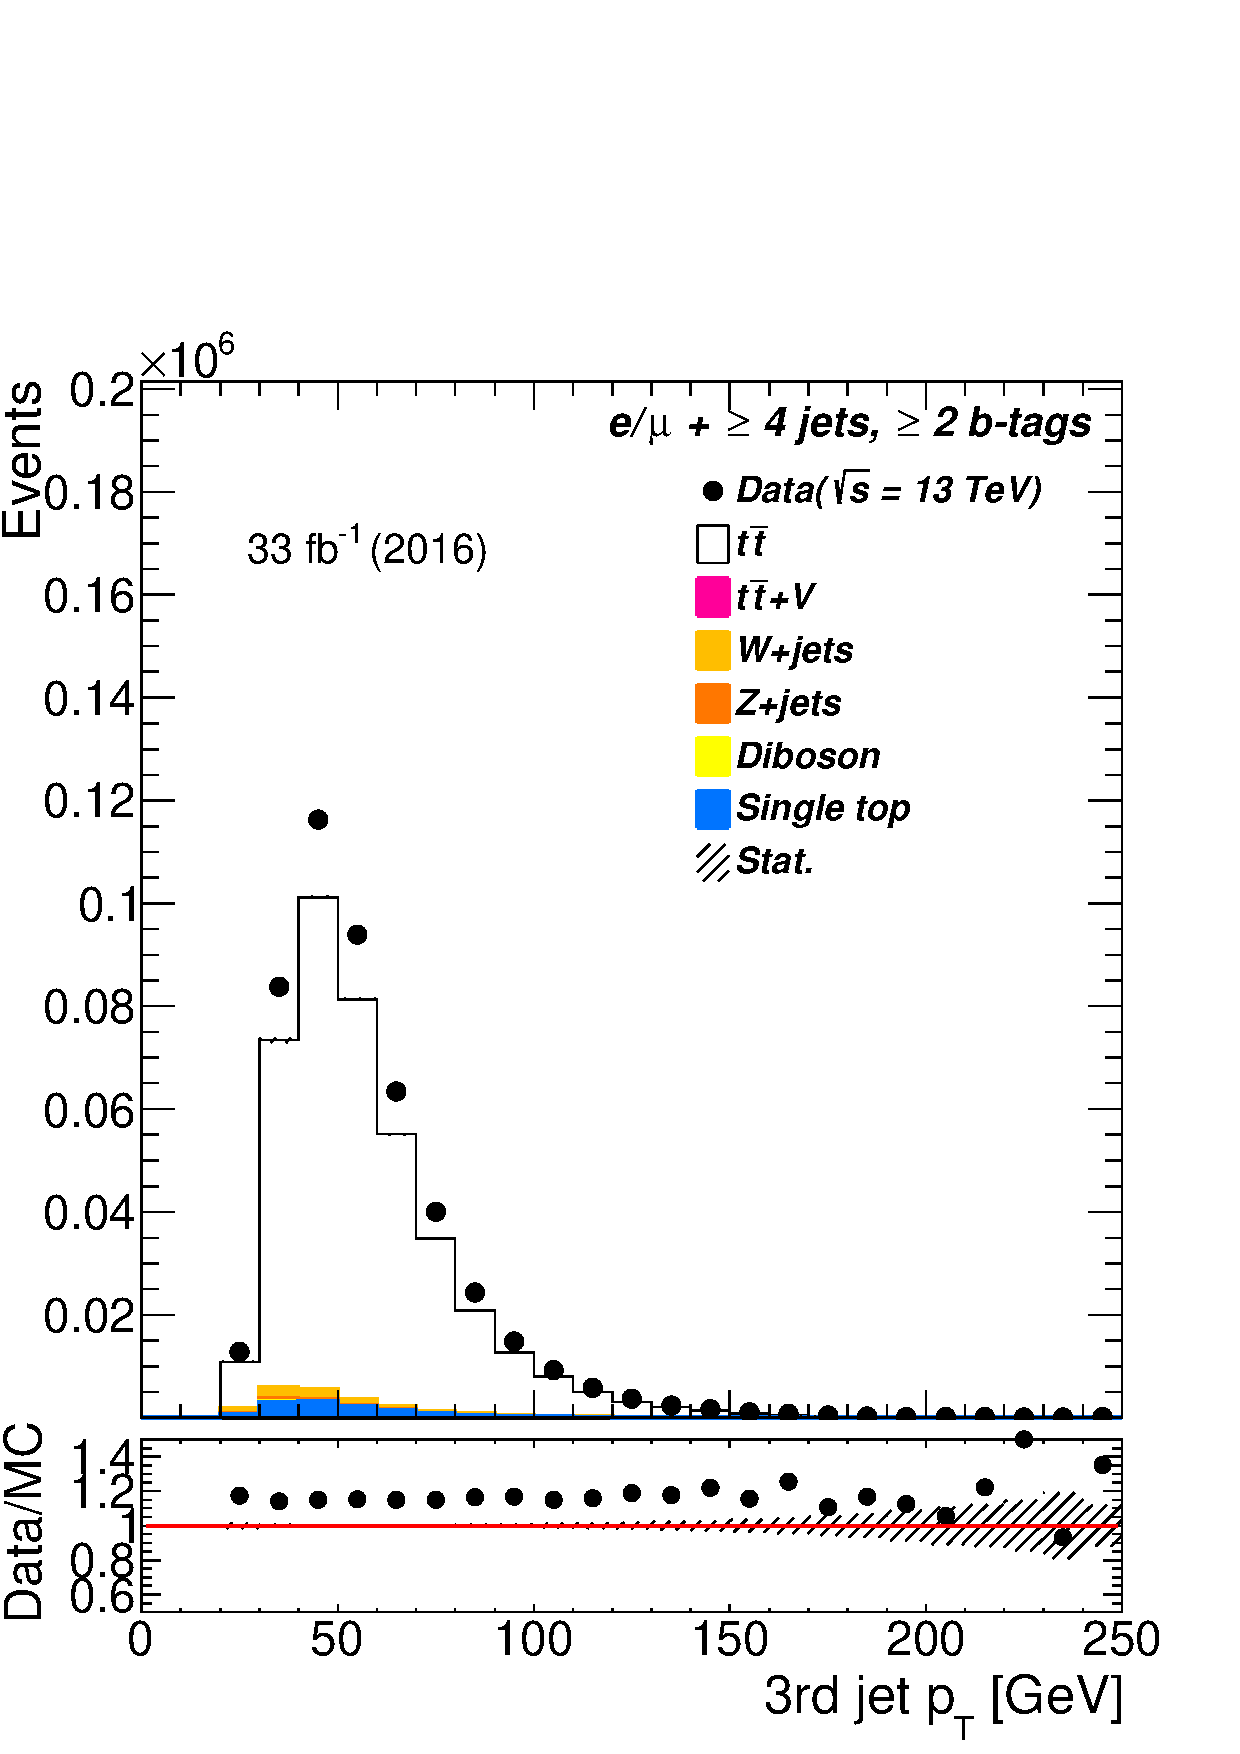
\includegraphics[width=\linewidth]{ControlPlots_emujets_2016_4incl_2incl/jet2_pt_emujets_2016.png}
	\caption{Transverse momentum of the third jet.} \label{fig:4a}
  \end{subfigure}



\begin{subfigure}{0.25\textwidth}
	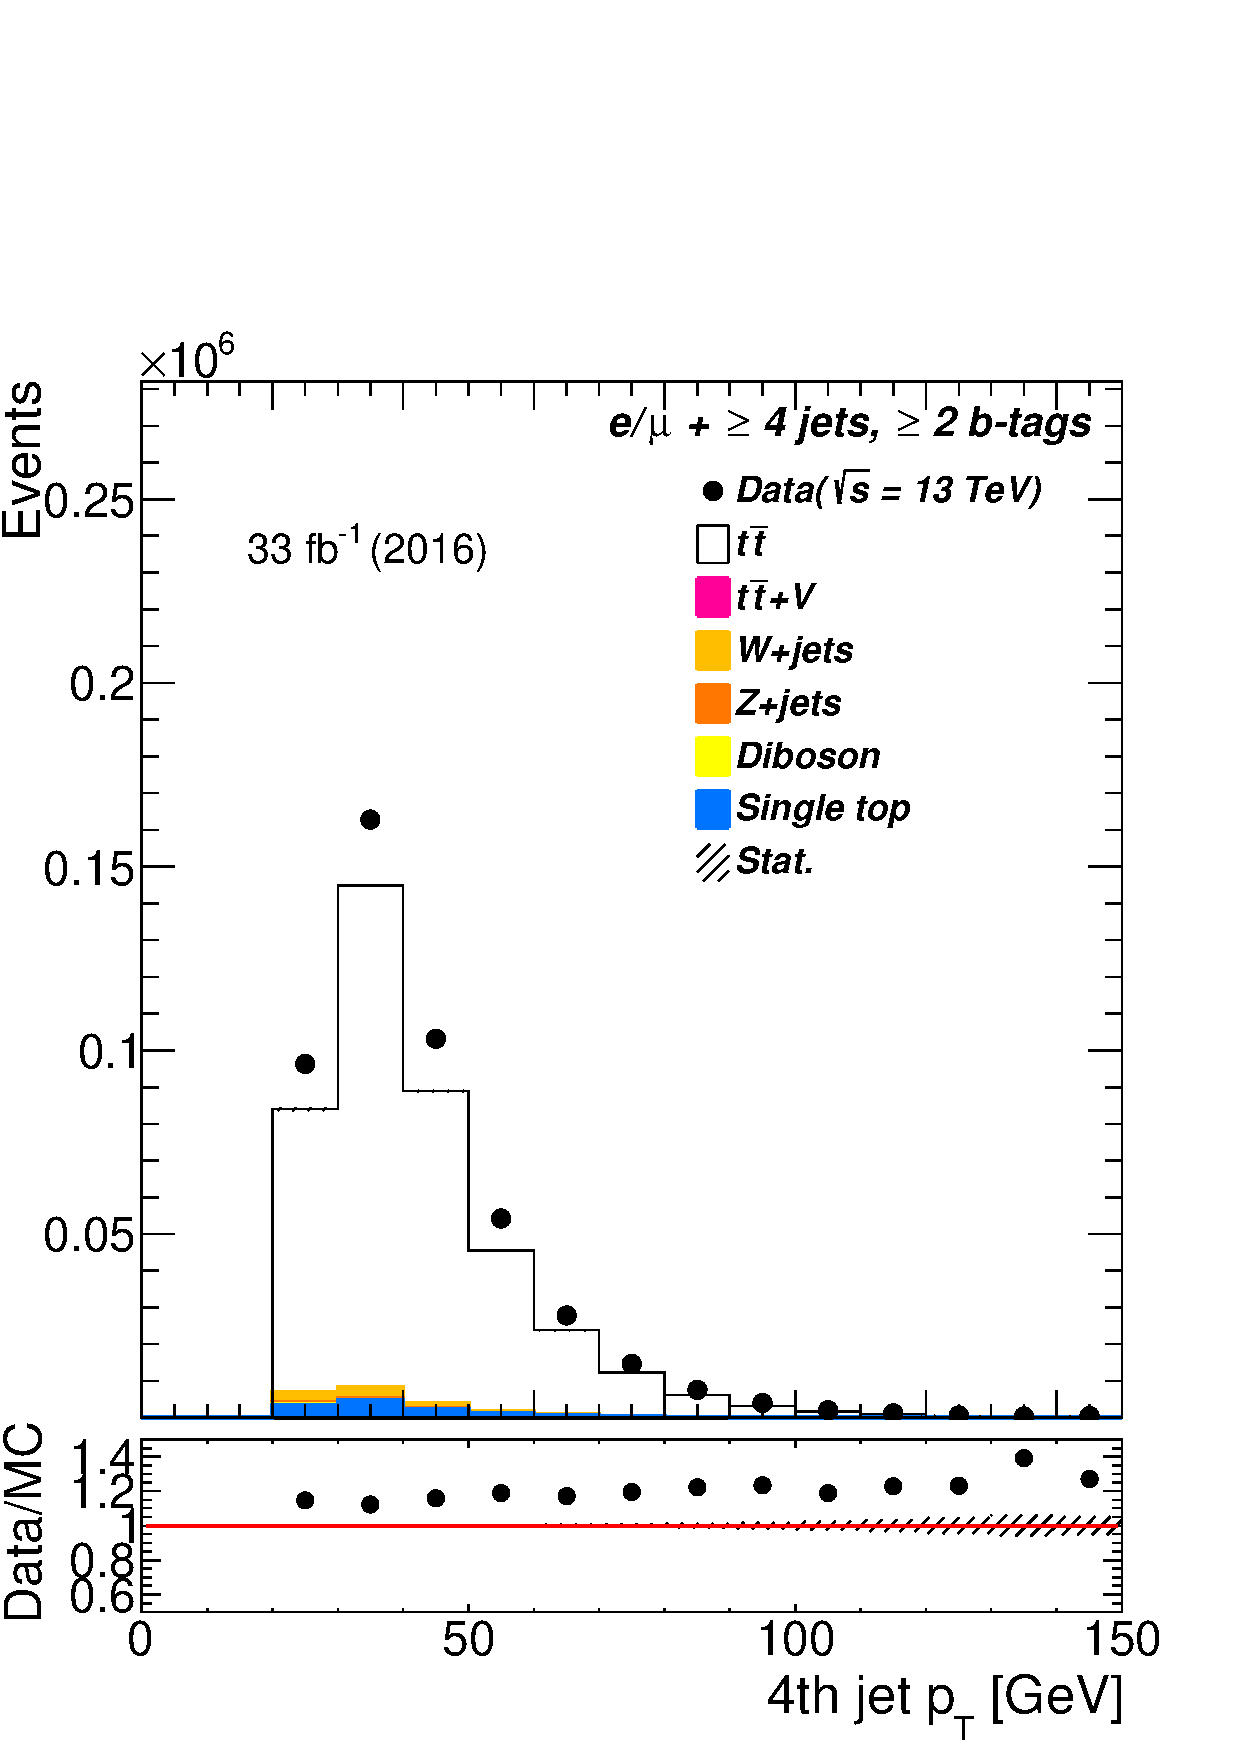
\includegraphics[width=\linewidth]{ControlPlots_emujets_2016_4incl_2incl/jet3_pt_emujets_2016.png}
	\caption{Transverse momentum of the fourth jet.} \label{fig:4xb}
\end{subfigure}\hspace*{1.0cm}
\begin{subfigure}{0.25\textwidth}
	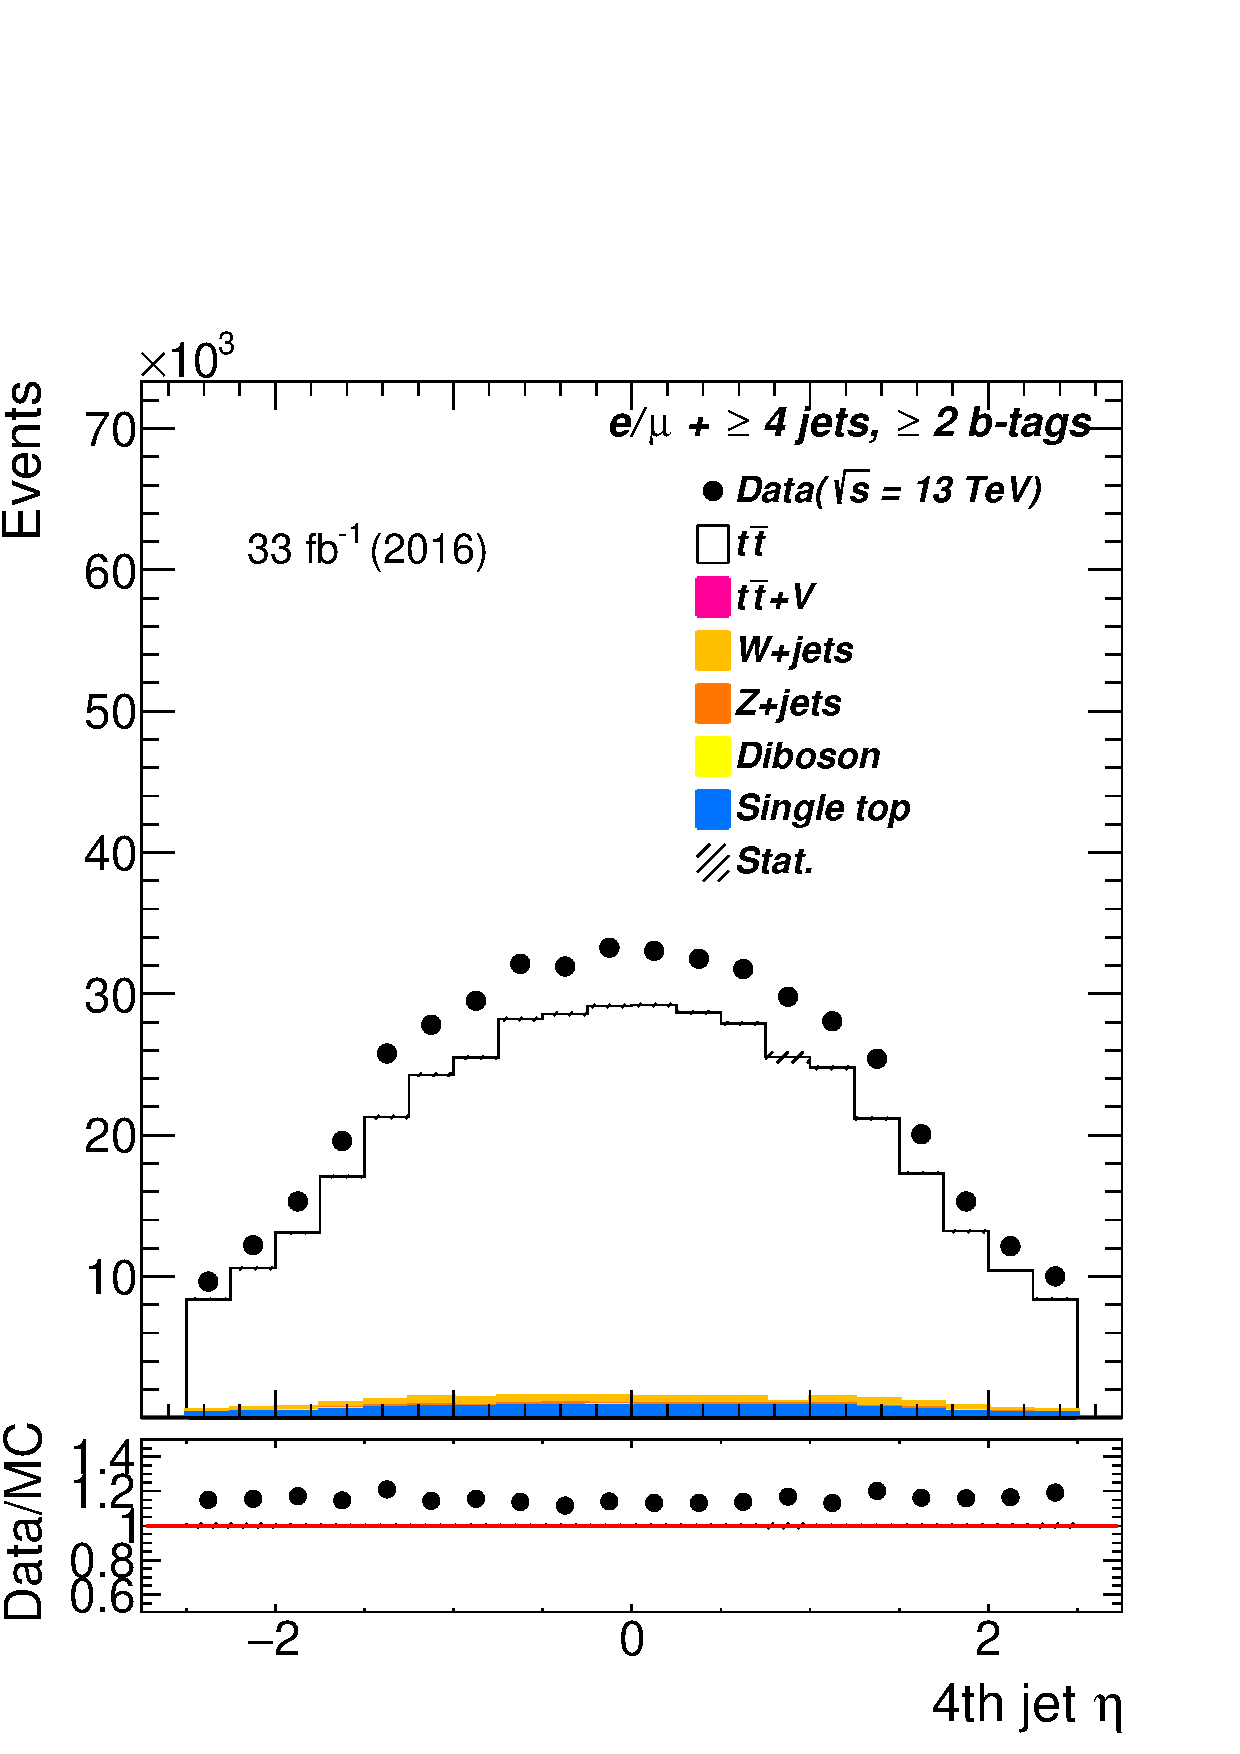
\includegraphics[width=\linewidth]{ControlPlots_emujets_2016_4incl_2incl/jet3_eta_emujets_2016.png}
	\caption{Rapidity of the fourth jet.} \label{fig:4dc}
\end{subfigure}\hspace*{1.0cm}
\begin{subfigure}{0.25\textwidth}
	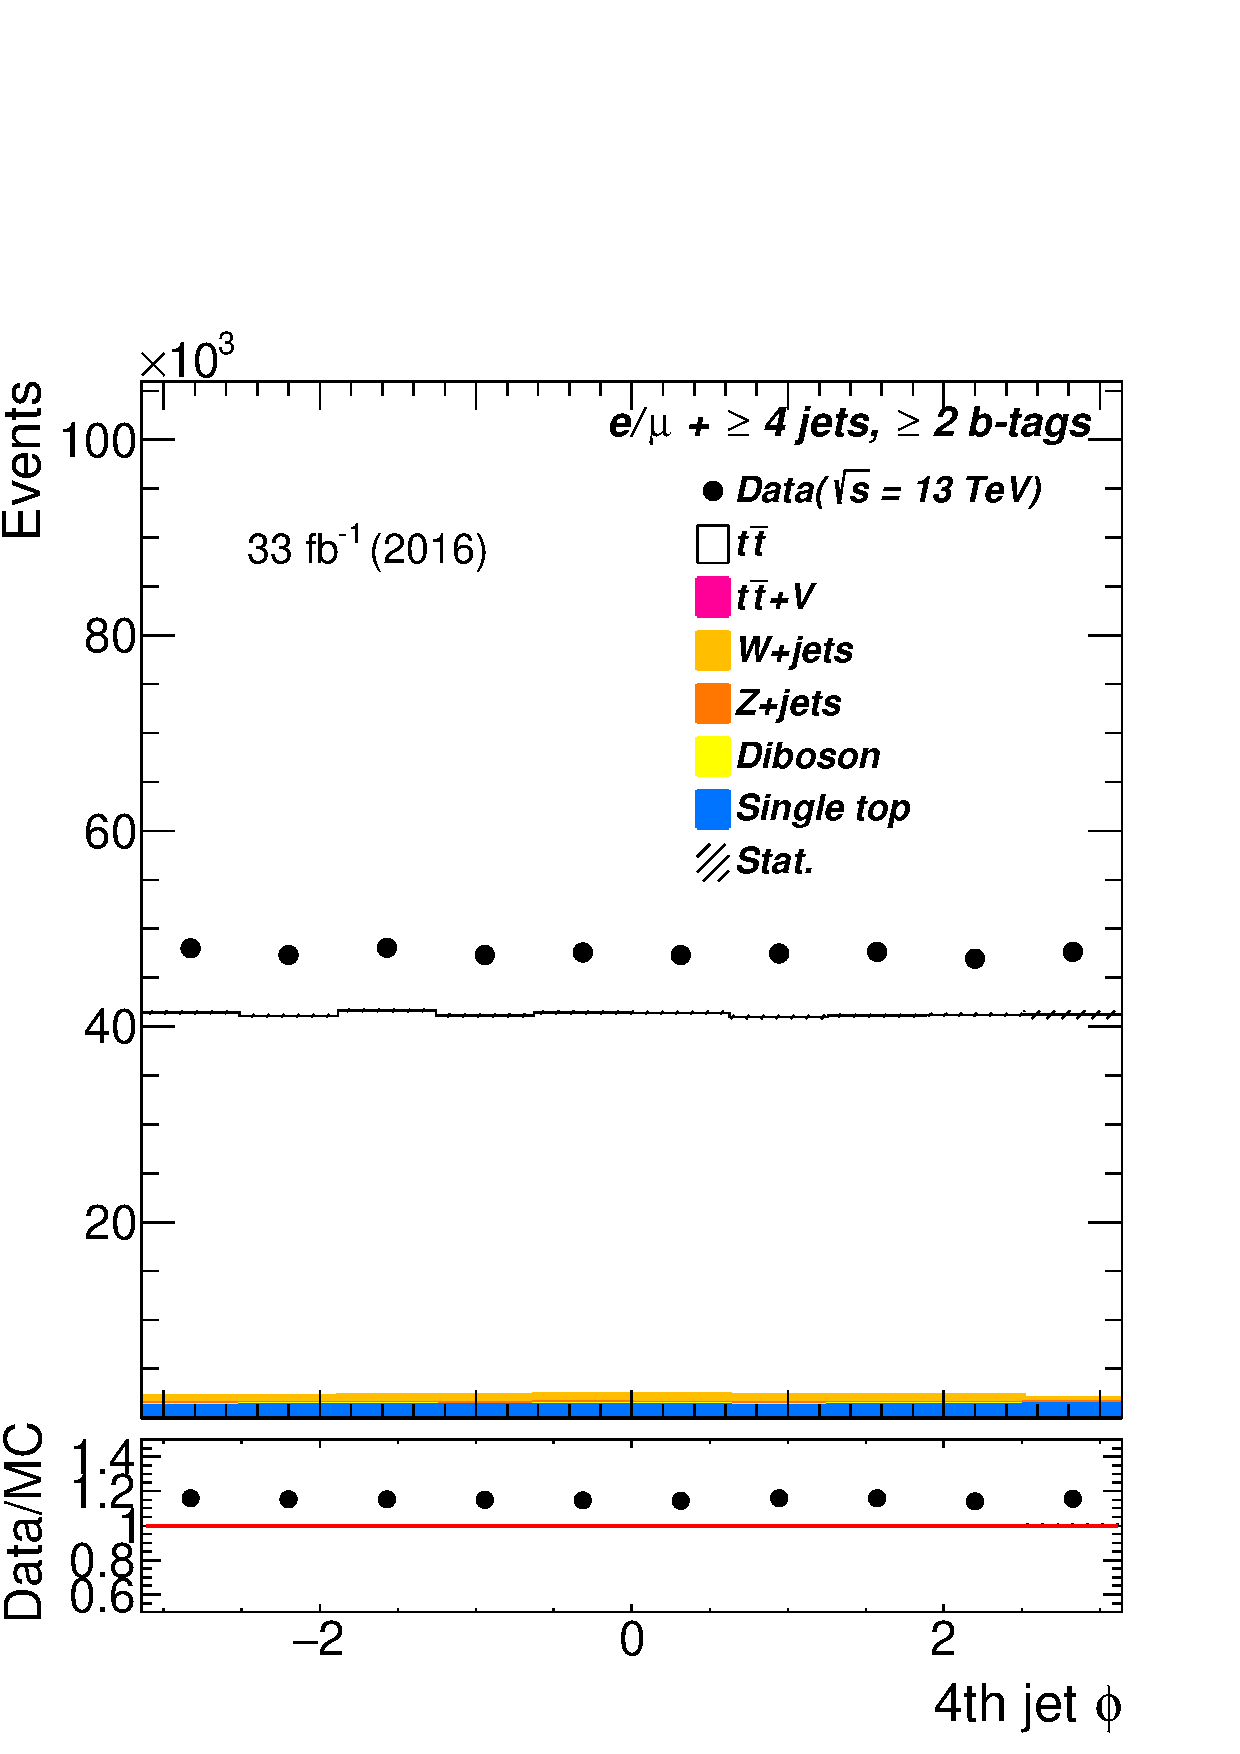
\includegraphics[width=\linewidth]{ControlPlots_emujets_2016_4incl_2incl/jet3_phi_emujets_2016.png}
	\caption{$\phi$ of the fourth jet.} \label{fig:4dd}
\end{subfigure}


\caption{Global quantities of the second and the third jet, obtained for the one $b$-tag sample.}
\end{figure}	

